\documentclass[conference]{IEEEtran}
\usepackage{cite}
\usepackage{balance}
\usepackage{graphicx}
\usepackage{url}
\usepackage{subfigure}
\usepackage{verbatim}
\usepackage{fancyvrb}
\usepackage{enumitem}
\setitemize{noitemsep,topsep=2pt,parsep=1pt,partopsep=1pt}
\usepackage{multirow}
\usepackage{fancyvrb}
\usepackage{hyperref}
\usepackage{amsmath}
\usepackage{dcolumn}
\usepackage{color, colortbl}
\definecolor{Gray}{gray}{0.9}

\usepackage{xspace}
\newcommand{\ie}{{\emph{i.e.}},\xspace}
\newcommand{\viz}{{\emph{viz.}},\xspace}
\newcommand{\eg}{{\emph{e.g.}},\xspace}
\newcommand{\etc}{etc.}
\newcommand{\etal}{{\emph{et al.}}}
\newcommand{\GH}{{\sc GitHub}\xspace}
\newcommand{\Tvis}{{\sc Travis CI}\xspace}
\newcommand{\Tvi}{{\sc Travis}\xspace}
\newcommand{\CB}{{\sc CloudBees}\xspace}
\newcommand{\CCI}{{\sc CircleCI}\xspace}
\newcommand{\DO}{{\sc DevOps}\xspace}
\newcommand{\Perc}{{\sc Perceval}\xspace}
\newcommand{\GLab}{{\sc GrimoireLab}\xspace}
\newcommand{\GHT}{{\sc GHTorrent}\xspace}
\newcommand{\TT}{{\sc TravisTorrent}\xspace}
\newcommand{\CI}{{$\mathcal{CI}$}\xspace}
\newcommand{\tdd}{{$\mathcal{TDD}$}\xspace}
\newcommand{\bCI}{{$\bm{\mathcal{CI}}$}\xspace}
\newcommand{\PR}{{$\mathcal{PR}$}\xspace}
\newcommand{\PRs}{{$\mathcal{PR}$s}\xspace}
\newcommand\head[1]{\noindent{\underline{\bf{#1}}:}}
\newcommand{\mypara}[1]{\vspace{4 mm} \noindent{\underline {\bf #1} \vspace{2mm}}}

\usepackage[table]{xcolor}
\usepackage{ifthen}
\usepackage{amssymb}

\newboolean{showcomments}
\setboolean{showcomments}{true} % toggle to show or hide comments
\ifthenelse{\boolean{showcomments}}
  {\newcommand{\nnbb}[2]{
    \fcolorbox{gray}{yellow}{\bfseries\sffamily\scriptsize#1}
    {\sf\small$\blacktriangleright$\textit{#2}$\blacktriangleleft$}
   }
   \newcommand{\version}{\emph{\scriptsize$-$working$-$}}
  }
  {\newcommand{\nb}[2]{}
   \newcommand{\version}{}
  }
%\newcommand{\as}[1]{\nnbb{Alexander}{#1}}
%\newcommand{\bv}[1]{\nnbb{Bogdan}{#1}}
%\newcommand{\vf}[1]{\nnbb{Vladimir}{#1}}
%\newcommand{\yz}[1]{\nnbb{Yangyang}{#1}}
\newcommand{\as}[1]{}
\newcommand{\bv}[1]{}
\newcommand{\vf}[1]{}
\newcommand{\yz}[1]{}

\newcommand\blfootnote[1]{%
  \begingroup
  \renewcommand\thefootnote{}\footnote{#1}%
  \addtocounter{footnote}{-1}%
  \endgroup
}

\VerbatimFootnotes

\begin{document}

%\title{How Do Software Development Practices
%Change Following Adoption of Continuous Integration?}
\title{The Impact of Continuous Integration on \\Other Software 
Development Practices: \\A Large-Scale Empirical Study}


\author
{\IEEEauthorblockN{Yangyang Zhao$^*$}
\IEEEauthorblockA{Nanjing University\\ China\\njuzhyy@gmail.com}
\and
\IEEEauthorblockN{Alexander Serebrenik}
\IEEEauthorblockA{Eindhoven U of Technology\\ The Netherlands\\a.serebrenik@tue.nl}
\and
\IEEEauthorblockN{Yuming Zhou}
\IEEEauthorblockA{Nanjing University\\ China\\zhouyuming@nju.edu.cn}
\and
\IEEEauthorblockN{Vladimir Filkov}
\IEEEauthorblockA{UC Davis\\ USA\\filkov@cs.ucdavis.edu}
\and
\IEEEauthorblockN{Bogdan Vasilescu$^*$}
\IEEEauthorblockA{Carnegie Mellon University\\ USA\\vasilescu@cmu.edu}
}
\maketitle
\begin{abstract}
Continuous Integration (CI)
%\blfootnote{$^*$These authors contributed equally to this work} 
%has become a key part of the modern ideology 
%of mashing development and operations together to shorten the cycles of 
%delivering a product to users. 
%CI 
has become a disruptive innovation in software development: with proper 
tool support and adoption, positive effects have been demonstrated for pull 
request throughput and scaling up of project sizes. 
As any other innovation, adopting CI implies adapting existing practices in 
order to take full advantage of its potential, and ``best practices'' to that end 
have been proposed. 
Here we study the adaptation and evolution of code writing and submission,
issue and pull request closing, and testing practices as \Tvis is adopted by 
hundreds of established projects on \GH. 
Qualitatively, to help essentialize the quantitative results, we survey a 
sample of \GH developers about their experiences with adopting \Tvis. 
Our findings suggest a more nuanced picture of how \GH teams are adapting to, and
benefiting from, continuous integration technology than suggested by prior
work.
\end{abstract}

% !TEX root = CI_Adoption.tex

\section{Introduction}

It is not everyday that software engineering experiences a paradigm shift.
The \DO movement, made popular in recent years, is according to many
\cite{degrandis2011devops, loukides2012devops, humble2011enterprises, 
roche2013adopting} such a shift.
Simply stated, \DO aims to get changes into production as quickly as 
possible, without compromising software quality.
While no standard definitions exist and the term is often overloaded, here
we refer to \DO as a culture that emphasizes \emph{automation of the 
process of building, testing, and deploying software}.
In practice, \DO is supported by a multitude of configuration management, 
cloud-based continuous integration, and automated deployment tools,
which enjoy widespread open-source~\cite{Hilton2016} and industrial 
adoption~\cite{rightscale, hilton2016continuous}.

In this study we focus on Continuous Integration (CI), the key enabler of \DO.
CI is a well known concept in Extreme Programming, often attributed to
Martin Fowler's 2000 blog post~\cite{fowler2000continuous}.
As a practice, CI is seeing broad adoption with the increasing popularity
of the \GH pull-based development model~\cite{gousios2014exploratory}
and the plethora of open-source, \GH-compatible, cloud-based CI 
tools,\footnote{\url{https://github.com/integrations/feature/continuous-integration}}
such as \Tvis, \CB, and \CCI.
In this decentralized, social coding context, CI is particularly relevant. 
By automatically building and testing a project's code base, in isolation, 
with each incoming code change (\ie push commit, pull request), CI 
has the potential to: (i)~speed up development (code change throughput)
\cite{Stolberg, pham2013creating, Hilton2016};
(ii)~help maintain code quality~\cite{VasilescuYWDF15, gousios2015work}.
Clearly, CI promises to be a disruptive technology in distributed software
development.
%However, despite its large scale adoption, we know relatively little about 
%the state of practice in using CI technology and the extent to which 
%developers are benefitting from its power.

For it to be effective, CI must allow for a seamless back and forth between
development, testing (\eg unit, integration, code review), and deployment. 
However, the road to efficiency is riddled with choices and trade-offs.
For example, working in large increments may lead to more meaningful
change sets, but it may also complicate synchronization between team 
members and, if necessary, reverting changes.
More frequent changes facilitate merging, but they also require more 
computing infrastructure for CI, since by default the code is built and all 
tests are executed with \emph{every} change.
Moreover, while CI runs on smaller, more frequent changes would provide 
earlier feedback on potential problems, they may also lead to process 
``noise'', where developers start to ignore the CI build status due to 
information overload, irrespective of whether the build is clean or 
broken~\cite{DeadCI}.

Several CI ``best practices'' have been proposed, \eg by Fowler in his 
influential blog post~\cite{fowler2000continuous}, such as 
\emph{Everyone Commits To the Mainline Every Day}, 
\emph{Fix Broken Builds Immediately},
and \emph{Keep the Build Fast}.
However, despite the large scale adoption of CI, we know relatively little 
about the state of the practice in using this technology and whether 
developers are benefitting from its power.

In this paper we report on a study of a sample of \GH open-source 
software projects that adopted \Tvis technology, by far the most popular 
CI infrastructure used on \GH~\cite{Hilton2016}.
In particular, we focus on the \emph{transition from no CI to using 
T{\footnotesize RAVIS} CI}, and investigate how development practices 
changed following the adoption of \Tvis.
Clearly, using CI seems beneficial.
But how much disruption does the transition to CI cause?
And how do teams change their workflows to accommodate CI?
Such knowledge can help developers to optimize their practices, project 
maintainers to make informed decisions about adopting CI, and 
researchers and tool builders to identify areas in need of attention.
To this end, we operationalize practices in three main aspects of 
distributed development, related to code changes, issue tracking, 
and testing.
To evaluate the effect of an intervention, in our case adoption of
\Tvis, on the transition toward expected behaviors in the above 
three practices (measured from trace data of \GH repositories),
we introduce \emph{regression discontinuity design analyses}.
Applying this methodology to hundreds of open-source Java 
projects, appropriately selected, we find that:


\begin{itemize}

\item There is a significant and persistent downward trend in commit churn after CI is adopted, over all projects, but also for a large fraction of individual projects. This trend is non-existent before the adoption.

\item Consistent with the above, we also find that the number of commits and PRs increases after CI adoption, and is random before it.

\item There is a rapidly increasing trend in the number of automatic test per PR after CI adoption.

\item There are significantly more issues submitted after CI adopted than before.

\item There are no significant changes in the frequency of commits after CI adoption.
\end{itemize}
\bv{Verify and update list of findings}

The remainder of this paper starts by developing the research questions pertaining to adoption of CI and its impact
 on developers' practices (Section~\ref{sec:background}), discusses the methods used to collect and analyze 
 the data (Section~\ref{sec:method}), presents the results (Section~\ref{sec:results}), reviews the related 
 work Section~\ref{sec:rw}), assesses threats to validity (Section~\ref{sec:threats}) and concludes 
 (Section~\ref{sec:conc}).

%In what follows, we tell this paper's story in a carefully crafted, yet mostly standard multisectioned format, beginning with the inimitable background and theory section, followed by an exemplary part on methodology, culminating in our tight results and logical discussion, with our long reaching conclusions, and the unavoidable threats to validity section bringing up the rear. \bv{Change this paragraph}

%sought to examine the extent to which best practices 
%of CI are actually transitioned to and followed, after CI adoption in online 
%software development projects. 
%We focus on three major aspects of modern development: practices 
%related to code changes, code testing, and code reviews \bv{Are we still doing reviews?}, and operationalize them into measures for them which we observe from trace data of GitHub repositories.
%We introduce regression discontinuity design analyses in order to 
%evaluate the effect of an intervention, in our case CI adoption, on the 
%transition toward expected behaviors in the above three practices.
%Applying those methods to hundreds of projects, appropriately selected, 
%we find that:

%https://sethrobertson.github.io/GitBestPractices/

%Devops, or bringing development and build/release activities in the same framework can bring changes in the product to the user-plane more quickly. For it to be effective, the technology that implements these ideas has to allow for a seamless back and forth between development, integration, code testing review, and release. 

%Continuous Integration is the part of devops that seamlessly builds, tests, and integrates developer changes, and performs any pre-specified testing. CI (\eg Travis CI, Jenkins CI, Hudson CI), if implemented properly, can benefit the distributed software development process, in particular code change throughput~\cite{Stolberg} and some aspects of code quality~\cite{VasilescuYWDF15}. It is a disruptive technology, in that it can scale up distributed development without noticeable diminishment in quality.

%Proper implementation is key here, otherwise the benefits may not be felt, and the technology may become a drag on resources, since it subsumes continuous builds and testing. 
%This is particularly true in team environments, where it falls to each individual developer to keep up with project specific implementation policies.
%For that reason, Martin Fowler wrote an article on CI best practices~\cite{}, which has been very influential and in many projects there are expectations that those practices define CI and that they will be followed.~\cite{}
%In particular, those practices are: Maintain a Single Source Repository,  Automate the Build, Make Your Build Self-Testing, Everyone Commits To the Mainline Every Day, Every Commit Should Build the Mainline on an Integration Machine, Fix Broken Builds Immediately, Keep the Build Fast, Test in a Clone of the Production Environment, Make it Easy for Anyone to Get the Latest Executable, Everyone can see what's happening, and Automate Deployment.
%But to what extent are they followed in practice?


% !TEX root = CI_Adoption.tex

\section{Development of Research Questions}
\label{sec:background}

%For a developer not proficient with the operational side of the process, 
Transitioning to an integrated CI platform, like \Tvi, involves adaptation 
of established processes to the new environment. 
During this transition, some developers will experience a more streamlined 
process evolution trajectory than others. 
Studying those trajectories can provide lessons learned.


%We expect the following to potentially change in the transition <need to write theory behind each>:
%
%On the developer side:
%Change in code writing/committing: we expect smaller change sets over time
%We expect More unit testing over time
%Operations side:
%More discussions in code review over time
%Different categories of initial faults


Continuous integration encourages developers to ``break down their work 
into small chunks of a few hours each'', as smaller and more frequent commits 
helps them keep track of their progress and reduces the debugging effort~\cite{Fowler,Duvall}. 
%The size of commits is closely related to commit frequency: indeed, the 
%aforementioned quote from Fowler's blog post refers to ``chunks of a few hours each''. 
Miller has observed that, on average, Microsoft developers 
committed once a day, while off-shore developers committed less frequently 
due to network latencies~\cite{Miller}; Stolberg expects everyone to commit every 
day~\cite{Stolberg} and Y\"{u}ksel reports 33 commits per day after introduction 
of CI~\cite{Yuksel}. On a related note, the interviewees in the study of 
Leppanen \etal~\cite{Leppanen2015} saw higher release frequency as an
advantage and reported that the CI ``radically decreased time-to-market''. 
Hence, we ask in \textbf{RQ1}: 
\emph{Are developers committing code more frequently?}

Frequent commits can be expected to be smaller in size: indeed, 
 the quote from Fowler's blog post refers to ``small chunks''~\cite{Fowler,Duvall}.
%Duvall [p. 31,38,40]
Hence, we formulate \textbf{RQ2}: 
\emph{Are developers reducing the size of code changes in each commit 
post CI adoption? 
Do they continue to do so over time?}

In the \GH-common pull-based development model, wherein project outsiders 
(and sometimes insiders too) submit changes in the form of pull requests (PRs), 
evaluation throughput is key.
Indeed, popular \GH projects receive increasingly many PRs, all of which need 
to be tested and reviewed pre-merge.
One of the most commonly advocated benefits of \Tvis is the ability to ``scale up'' 
development, by automating PR testing and delegating the workload to cloud-based
infrastructure; in this sense, Vasilescu \etal~\cite{VasilescuYWDF15} report that 
\GH teams are able to process (\ie close) more PRs per unit time after adopting \Tvis.
This high level of automation should also impact the speed, not just the volume, of
PR evaluations.
%Given all this automation, are PR evaluations also quicker, not just more numerous?
Hence, we ask in \textbf{RQ3}: 
\emph{Are pull requests closed more quickly post CI adoption?}

For CI, and \DO in general, to have the stated benefits, effective coordination
between all project contributors is important; a common mechanism for this
are issue reports.
Similarly to the pull requests, the number of closed issues per time period may change 
after CI adoption, in response to
increased project activity or efficiency. %, \eg related to code churn and automated testing.
%In the very popular pull-request model of development, code review is done through open issues.
%\as{Can we say something about the popularity of the pull-request model of development in GH? Is this your work or GG's?} 
%However, maintaining the process of code review has been recognized as one of 
%the challenges when adopting continuous deployment~\cite{ClapsBSA}, software 
%development technique related to continuous integration.
Hence, we ask in \textbf{RQ4}: 
\emph{Are more issues being closed after adopting CI?}
%\emph{Are developers transitioning to opening more or fewer issues after 
%adopting CI?}

Finally, CI is closely related to the presence of automated tests~\cite{Fowler}. 
Duvall even claims that CI without such tests should not be considered CI 
at all~\cite{Duvall}, while Cannizzo \etal~deem an extensive 
suite of unit and acceptance tests to be an essential first step~\cite{CannizzoCluttonRamesh}. 
Moreover, CI is frequently introduced together with test automation~\cite{Yuksel}.
However, developing tests suited for automation requires a change in developers' 
mindset, and presence of a comprehensive set of tests incurs additional maintenance 
costs~\cite{CoramBohner}.
Naturally, more automated testing will expose more errors, and CI makes it possible 
to track and react to different error types differently~\cite{BellerGZ16}.
%\as{Y\"{u}ksel reports increase of the number of automated tests but they have combined introduction of CI with automated testing~\cite{Yuksel}. }
Therefore, we formulate \textbf{RQ5}: 
\emph{How does the usage of automated testing change over time after CI adoption?} 
%And how do build errors evolve over time?}
%\as{Not sure about the formulation; the word ``transition'' implies that in the beginning the developers do not use automated testing. Do we really check this?}

%\subsection{RQs}

% !TEX root = CI_Adoption.tex

\section{Methods}
\label{sec:method}

We collected and statistically analyzed data from a large sample of open-source 
projects on \GH, that adopted \Tvis at some point during their history.
We further surveyed a sample of those projects' \Tvis adopters.
%Java (language chosen based on familiarity of the first author) 

\subsection{Data Gathering}

Data collection involved mining multiple sources: \GHT~\cite{gousios2012ghtorrent}, 
the \GH API, project version control (git) logs, and the \Tvis API.
The goal was to select non-trivial projects that adopted \Tvis, and had sufficient
activity both before and after adoption, in order to observe potential transition effects.
Note that for the purpose of this study we don't distinguish between ``project'' 
and ``repository''; the term ``project'' has also been used to refer to a collection 
of interrelated repositories in the literature~\cite{vasilescu2016sky}.

\smallskip\noindent\emph{Candidate Projects} 

We started by identifying \GH projects that use \Tvis.
To our knowledge, no such general list exists 
(\TT~\cite{beller2017travistorrent} is restricted to Java and Ruby projects), so
we wrote a script that iterates over non-fork \GHT projects (oldest to newest)
and pokes the \Tvis API (cf.\ \cite{era14}) to determine if the project used \Tvi;
we ran and stopped the script after identifying approximately half (165,549)
of all \GH projects that ever used \Tvis.\footnote{At the time of writing, \Tvi self 
reports being used in over 318,000 open source \GH projects, see 
\url{https://travis-ci.org}.} 

Next, we cloned the \GH repositories of all these projects locally, and extracted
their main-branch commit histories using \Perc, an open-source repository
mining tool part of the \GLab tool suite.\footnote{\url{http://grimoirelab.github.io}}
Following, we traversed each project's commit history to determine when 
maintainers introduced \Tvis, by identifying the earliest commit of the 
\texttt{.travis.yml} configuration file, and recorded its authored timestamp as
the timestamp of the \Tvi adoption.

\begin{figure}[t]
	\centering
	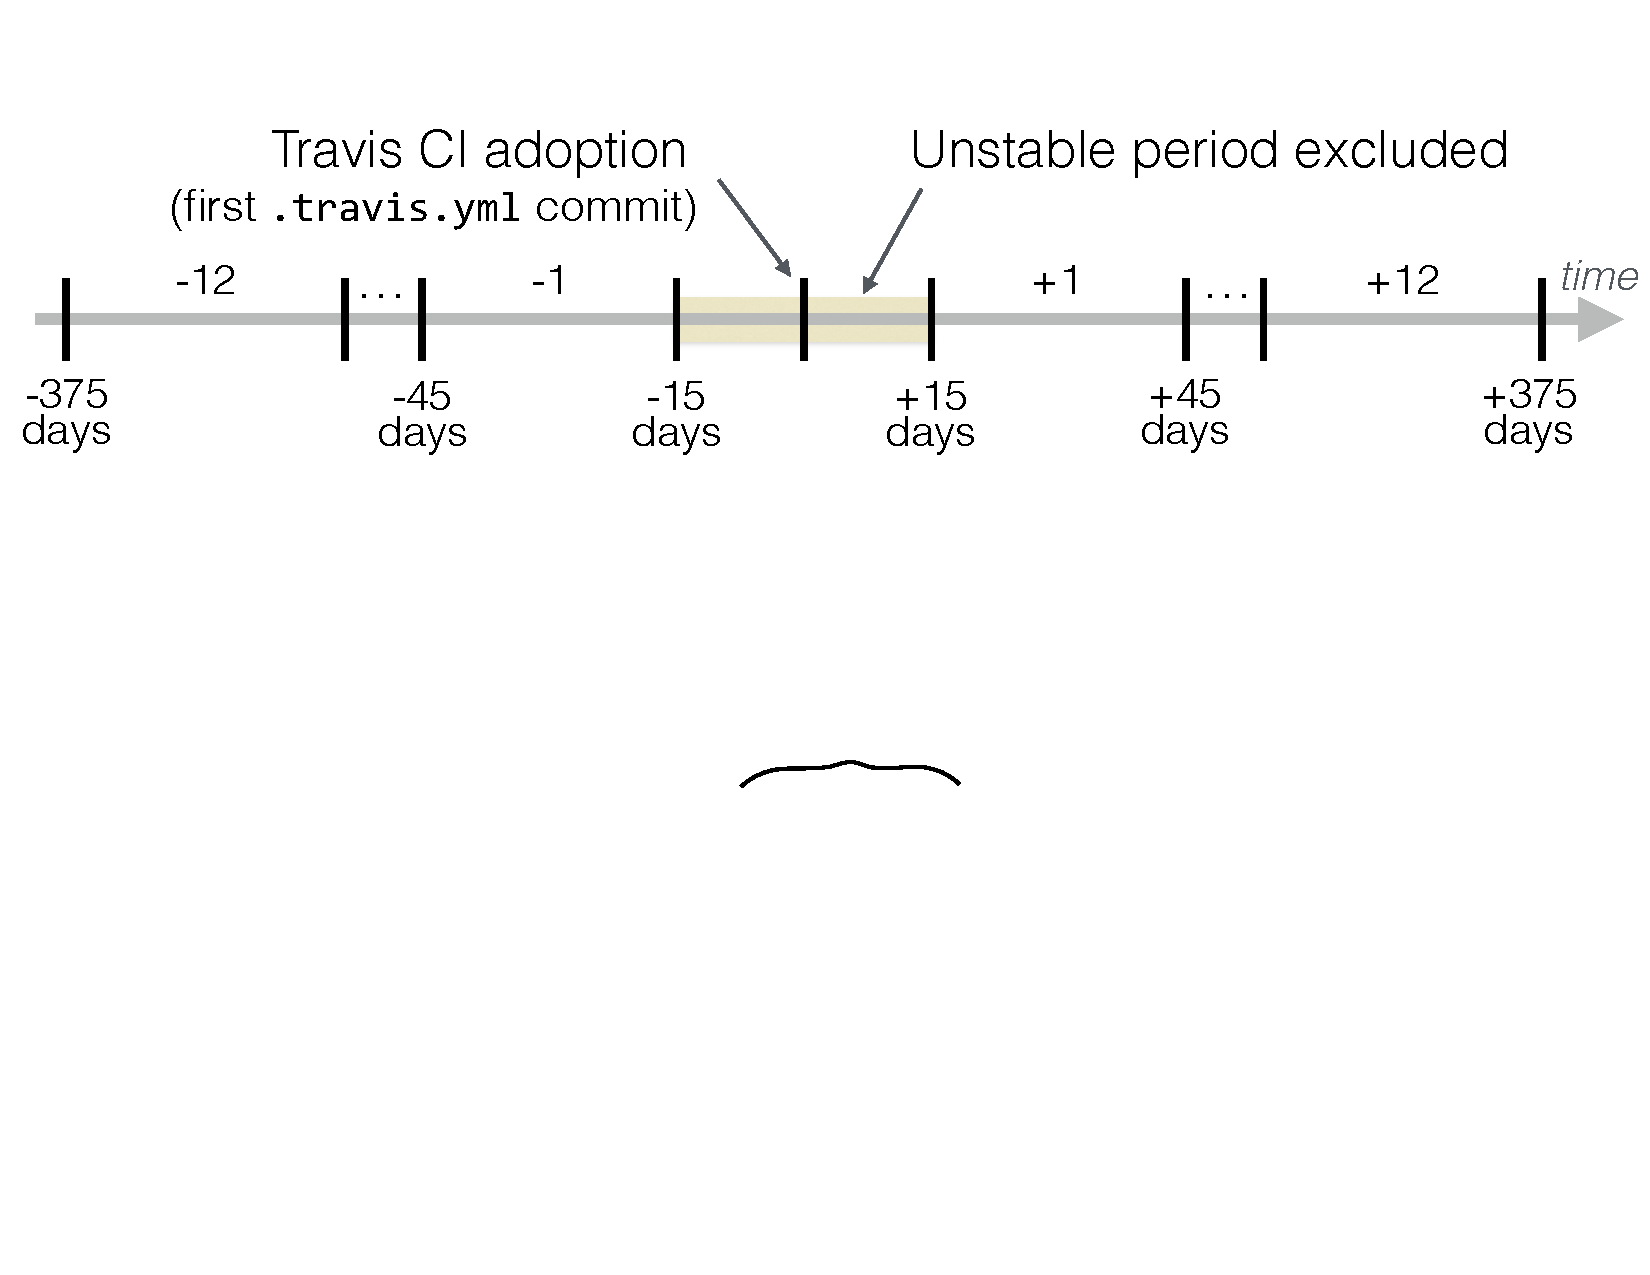
\includegraphics[width=\columnwidth, clip=true, trim=0 392 0 40]{figures/timeline.pdf}
	\caption{Overview of our time series assembly method.}%\vspace{-0.5cm}
	\label{fig:timeseries}
\end{figure}

\smallskip\noindent\emph{Time Series}

We proceeded to aggregate data about the different practices considered
in 30-day windows, 12 on each side, around the \Tvis adoption event
(Figure~\ref{fig:timeseries}).

During initial exploration, we observed that on several occasions \Tvi has 
been adopted as part of a larger restructuring effort, which lasted several days.
Examples include changing the build system from Ant to Gradle and, 
consequently, how project folders are organized; updating library 
dependencies; and restructured tests.
Based on this anecdotal evidence, we concluded that the activity immediately 
prior to and immediately following the introduction of \Tvis might not be 
representative of the project's overall trends.
Therefore, to limit the risk of bias due to extraordinary project activity in 
the transition period, we excluded one month of data centered around the 
adoption event in our quantitative analyses below.

\smallskip\noindent\emph{Measures}

We collected global and time-window-specific measures: 
\begin{itemize}

\item \textbf{total number of commits} in a project's history, as a proxy for 
project size / activity.

\item \textbf{total number of commit authors}, as a proxy for the size of a
project's community; commit authors include both core developers, who are
also committers, and external contributors, without ``write'' access, whose 
commits are merged in by the core developers.
Since it is common for open-source developers to contribute under different 
aliases (name-email tuples), \eg as a result of using different machines and 
changes in git settings over time, we first performed \emph{identity merging}.
We used heuristics that match first and last names, email prefixes, and email 
domains, cf.\ prior work~\cite{bird2006mining, vasilescu2015msrdata}, and
found an average of 1.15 (max 7) aliases per person in our dataset.

\item \textbf{project age} at the time of adopting \Tvis, in months, computed
since the earliest recorded commit.

\item \textbf{main programming language}, automatically computed by \GH
based on the contents of each repository and extensions of file names therein.

\item \textbf{number of non-merge commits}, \textbf{number of merge commits} 
per time window.
%, our measure of commit frequency.
Since git is a distributed version control system, developers can work locally,
in increments, before pushing their changes to \GH or opening a pull request.
E.g., a developer can choose to partition a large change into many smaller 
ones, and make multiple local commits to better manage the work.
This would not have any effect on CI runs, since CI is only triggered by \GH 
\emph{push} events, and events happening after (and including when) a pull 
request is opened.
%Pull requests are also a mechanism to isolate individual developers from 
%activity on the mainline.
Consequently, to study \emph{Commits To the \_Mainline\_ Every Day}
(Fowler's best practice), as opposed to potentially local git commits, we
distinguish between \emph{non-merge commits} and \emph{merge commits}
as a proxy.
We recognize non-merge commits as those having at most one parent, and
merge commits otherwise.

%\item  per time window.
%, as a proxy for how
%distributed a project's development is, over branches and forks.

\item \textbf{mean commit churn} for non-merge commits, per time window,
our measure of commit size.
Churn is computed as the total number of lines added plus the total number
of lines removed per commit (in git modified lines appear as first removed, 
then added), extracted from git logs.
The mean is computed over all non-merge commits commits in that time window.

\item \textbf{number of issues opened / closed}, \textbf{number of pull requests
opened / closed} per time window, extracted using the \GH API.

\item \textbf{mean pull request latency} per time window, in hours, computed 
as the difference between the timestamp when the PR was closed and that 
when it was opened.
The mean is computed over all PRs in that time window.
\end{itemize}

\bv{Add something about build logs and unit tests.}
%(i)~its history of commits, issues, and pull 
%requests using the \GH API; and 
%(ii)~its history of \Tvis builds and, for each
%build, all its job logs (a \Tvis build can be configured to run multiple jobs,
%one for each set of user-defined configuration options; each job run produces 
%a ``build log''), using the \Tvis API and the \textit{travis gem} Ruby library.  


\smallskip\noindent\emph{Filtering}

As a large fraction of projects on \GH are small and not highly 
active~\cite{gousios2014exploratory}, we filtered out projects that had not 
been consistently active during our 24-month observation period: we require
at least one commit on the main branch in each of the 24 time windows 
(in our sample only 2,595 projects, across 83 programming languages, satisfy 
this requirement).
Furthermore, our multivariate regression analysis below requires enough 
variance along each of the dimensions being modeled, thus we additionally
filter out programming languages not represented by at least 10 projects each.
The resulting dataset consists of 2,446 projects across 22 languages.

\bv{Talk about outlier removal}

\bv{Add dataset overview table}

% !TEX root = ../CI_Adoption.tex

\begin{table}[t] \centering
\small
  \caption{Examples for the outputs in terms of MAVEN, GRADLE and ANT
  \vspace{-0.2cm}
  }
  \label{log_example}

\begin{tabular}{ p{8cm}}
	\hline
	\\[-1.8ex]\hline
		\textbf{MAVEN}         \\
		\begin{tabular}[c]{@{}l@{}}
			\textit{-------------------------------------------------------}\\ 
			\textit{ T E S T S}\\ \textit{-------------------------------------------------------}\\ 
			\textit{Running org.sonar.ide.intellij.inspection.InspectionUtilsTest}\\ \textit{Tests run: 1, Failures: 0, Errors: 0, Skipped: 0, Time elapsed:}\\ \textit{0.202 sec}\\ 
			\textit{Results:}\\ 
			\textit{Tests run: 1, Failures: 0,Errors: 0, Skipped: 0}\end{tabular} \\  \hline
	
		\textbf{ANT}          \\
		\begin{tabular}[c]{@{}l@{}}
			\textit{{[}junit{]} Running limelight.BufferedImagePoolTest}\\ 
			\textit{{[}junit{]} Testsuite: limelight.BufferedImagePoolTest}\\ \textit{{[}junit{]} Tests run: 5, Failures: 0, Errors:0, Time elapsed: 0.143 sec}\end{tabular}                                                                                                                                                \\  \hline
		\textbf{GRADLE}          \\
		\begin{tabular}[c]{@{}l@{}}
			\textit{:test}\\ 
			\textit{...}\\ 
			\textit{1 test completed, 1 failed}\\
			\textit{:test FAILED}\\ 
			\textit{Total time: 3.8 secs}\end{tabular}      \\ \hline                                                                                                                                                                                                                                                
	\end{tabular}
\end{table}

\smallskip\noindent\emph{Number of Tests Executed per Build} 

We also parsed the \Tvis build logs and extracted information about the 
number of tests executed. % and the types of reasons causing builds to break.
%We provide more details next.
Each \Tvis build consists of at least one job, which corresponds to a particular
build and test environment (\eg jdk version, environment variables). 
Once the job is started, a log is generated, recording the detailed information
of the build lifecycle, including installation steps and output produced by the 
build managers. % scripts for testing. 
Table~\ref{log_example} shows fragments of the logs generated by the 
three widely used Java build tools, Maven, Ant, and Gradle. 
To investigate the evolution in testing practices across builds, we wrote a tool 
to analyze the logs and extract summary information about test executions.  
Since the relationship between builds and jobs is one-to-many, we use the 
maximum number of tests across jobs as the test count for the build. 



%We started by composing (using the \GH Search API) a list of candidate Java 
%projects that: (i)~were not very small (a large fraction of projects on \GH are 
%small and inactive~\cite{gousios2014exploratory}; we arbitrarily chose to ignore
%projects smaller than 500 kilobytes, using the \GH Search API's \emph{size} 
%parameter); and (ii)~were created no later than 2014-11-08. 
%The second criterion is a consequence of our data collection date (2016-05-01)
%and the ``sufficient history'' requirement. 
%Our statistical analysis, detailed below, assumes 9 months of history for each
%project both prior to and after adopting \Tvis; since we did not have access to
%data on when each project started using \Tvis at this stage, we conservatively
%chose the 2014-11-08 date, which allows 9*30*2 days of history from project 
%creation to 2016-05-01.
%This step resulted in a list of over 300,000 candidate Java projects.

%first and foremost, we should make sure our studied projects have sufficient history (e.g. 9*30 days) both before using Travis-CI and after using Travis-CI.  As the data were extracted from the inception until 2016-05-01, the projects selected should be created at least before 2014-11-08, so that there are at least 9*30*2 days from its creation to 2016-05-01. 
%From GitHub Search API, we first found over 300k Java projects created before 2014-11-08 and with $\geqslant 500$ kilobytes. 
%After consulting Travis-CI, we further identify projects that: 1) adopted Travis-CI; 2) at least 9 * 30 days from project creation to Travis-CI adoption; 3) at least 9 * 30 days from Travis-CI adoption to 2016-05-01. This filtering process left us 1566 projects.  
%For each project, we collect the whole history of commits, issues, and pull requests from GitHub API, and the history of Travis-CI builds and job logs from Travis-CI repository using the ruby library of \textit{travis gem}.  In addition to these publicly available data, we further gathered the information about the number of tests and types of errors during the Travis-CI run.

%Next, we used the \Tvis API to determine which of these projects:
%(i)~used \Tvis, and if yes, we recorded the date of the earliest build as the 
%adoption date; (ii)~had at least 9*30 days of history from project creation to 
%the adoption date, and from the adoption date to 2016-05-01, respectively. 
%This filtering process resulted in 1,566 projects.

%\smallskip\noindent\emph{Mainline commits:}
%
%Since git is a distributed version control system, developers can work locally,
%in increments, before pushing their changes to \GH or opening a pull request.
%E.g., a developer can choose to partition a large change into many smaller 
%ones, and make multiple local commits to better handle the work.
%This would not have any effect on CI runs, since CI is only triggered by \GH 
%push events, and events happening after (and including when) a pull request 
%is opened.
%%Pull requests are also a mechanism to isolate individual developers from 
%%activity on the mainline.
%Consequently, to study \emph{Commits To the \_Mainline\_ Every Day}
%(Fowler's best practice), as opposed to potentially local git commits, we
%distinguish between \emph{non-merge commits} and \emph{merge commits}
%as a proxy.
%We use  \texttt{\small git rev-list --all --merges} to recognize merge commits.

%Starting from RQ1 and RQ2 the practice being investigate should be �Commits To the Mainline Every Day�, but then you analyze git commits. Not surprisingly, commits do not increase. Why they should? The main reason of having many commits is the ability to partition a large change in many smaller ones and to better handle the work locally. What really matters for the CI are pushes and pull requests. Indeed, I would expect an increase of pushes/pull requests when CI is being adopted. Maybe a way to observe this is to actually analyze merge commits and see whether their frequency increases.
%Similar considerations apply for the size of code changes. Also, I�ve the feeling that such a size may strongly depend on the kind of activity being performed. For example, it could be that bug fixing correlates with small change size, whereas feature addition with larger ones. 

%\smallskip\noindent\emph{Bug fixing vs.\ other activities:} 
%
%The kind of activity being performed may confound commit size, \eg since one 
%can expect bug fix commits to be smaller than new feature implementations.
%We additionally annotate the non-merge commits as \emph{bug-fixing} or not, 
%by searching for typical patterns in commit 
%messages~\cite{mockus2000identifying}.\footnote{E.g., \verb$^(bug)?fix(es|s|ed|ing)?(bug)?([[:punct:]]|\\s+)$}
%Note that we don't enforce that commit messages that match our regular
%expressions also contain references to existing issue report numbers, in an
%attempt to be more robust to different issue trackers (indeed, not all projects 
%use \GH's issue tracker) and different project linking / commit message conventions.
%%
%%The "fix" heuristic without issue tracker links (looking for issue numbers and verifying they exist in the issue tracker) has the disadvantage that it will detect "false positives", i.e., commits made not in response to an open issue; plus the extra disadvantage that it will identify commit messages containing "suffix", for example.
%%
%%However, not all projects use GitHub's issue tracker, as we know and a reviewer pointed out. Also, the original intent, triggered by a review comment, was to distinguish between new features and bug fixes. We can say that the "fix" heuristic more closely accomplishes this by being robust to issue trackers and project linking conventions. The only downside I can think of is if people close open "feature request" issues from the issue tracker, using "fix" language.
%



%% !TEX root = CI_Adoption.tex

\begin{table}[t] \centering
\small
  \caption{Travis-CI build failure taxonomy
  \vspace{-0.2cm}
  }
  \label{error_types}

\begin{tabular}{ p{1.5cm}  p{2.5cm}  p{4cm} }
	
\hline 
\\[-1.8ex]\hline
Category & Description & Examples of textual patterns \\ \hline 
\emph{failed test} & tests were failed & tests failed, TestsFailedException, tests unsuccessful\\ \hline
\emph{skipped or pending test} & tests were skipped or set to be pending & skipped tests \\ \hline
\emph{missing file or dependency} & required files or dependencies are not available &  FileNotFoundException, no such file to load, is not installed \\ \hline
\emph{code quality} & the code failed to satisfy the code standards & line too long, missing whitespace around operator, too many pylint violations \\ \hline
\emph{compile error} &compilation errors happened & Compilation failed, syntax check failed, attributeError, parse error\\ \hline
\emph{execution error} &an error occurs during the execution of code & runtime error, execution failed, test errors, OutOfMemoryError\\ \hline
\emph{time out} & the build could not be completed within the required time&“test run exceeded * minutes”, “..took longer than”, command time-out \\ \hline 
\emph{other} &other infrequent errors are included in this type & warnings on documentation, Aborted due to warnings, The remote end hung up unexpectedly \\
\hline

\end{tabular}

\end{table}



%\smallskip\noindent\emph{Error classification for failed builds:}
%
%\Tvis marks a build as \textit{failed} if at least one of its jobs not explicitly 
%labeled as \emph{allowed to fail} in the project's CI configuration 
%file\footnote{\url{https://docs.travis-ci.com/user/customizing-the-build/#Rows-that-are-Allowed-to-Fail}} failed.
%Therefore, to understand why \Tvis builds failed, we proceed to find out 
%what happened in the jobs. 
%We first manually reviewed a set of failed jobs to recognize what kinds of 
%failures occur and whether there are any corresponding textual patterns in 
%the logs.
%Then, we extracted a set of mapping rules to classify these patterns into 
%categories.
%We proceeded iteratively by inspecting more randomly selected failed jobs
%and gradually refining our classification scheme, until reaching saturation. 
%%To mitigate the risk of bias arising from missing and incorrect classification, 
%%we augmented the manual reviewing rates to improve our classification 
%%rules and remove spurious classification as much as possible. 
%%The classification scheme evolved during this process, and was gradually 
%%refined to cover more textual patterns. 
%In the end, we identified 8 categories of reasons for build failures, 
%as summarized in Table~\ref{error_types}. 
%%a group of mapping rules to classify the errors into 8 types, as shown 
%
%Next, we implemented tools for automatic classification. 
%The detailed process comprises the following steps:
%
%\noindent 1)~\emph{Failure Location}. 
%We first recognized failed jobs with \textit{non-allow-failure} attributes, which 
%result in the build's final \textit{failed} state. 
%Then, we attempted to locate the command which caused the breakdown 
%in the log file, as the command which exited with a non-zero value.
%The log entry for this command usually provided detailed information about 
%the fatal errors that occurred. 
%If such commands were not recorded in the log file, we expanded the search 
%scope to the \textit{script} phase and the \textit{after script} phase of the 
%build log, as per \Tvis build lifecycle.\footnote{\url{https://docs.travis-ci.com/user/customizing-the-build/#The-Build-Lifecycle}}
%Note that if errors occur in the \emph{before script} phase of the build, the 
%job is automatically marked as \textit{errored} and stops immediately. 
%Only if the \textit{script} phase returns a non-zero exit code, or the \textit{after 
%script} phase times out, then the job is marked as \textit{failed}. 
%Therefore, we first check if there is a time-out error in \textit{after script}. 
%If not, then it's likely that the errors in the \textit{script} phase caused the 
%build to break. 
%
%\noindent 2)~\emph{Log Parsing \& Tagging}. 
%After extracting the log fragment describing the errors, we 
%used textual pattern matching for classification. 
%%
%%\noindent 3)~\emph{Tagging}. 
%%We tagged the extracted textual patterns with a subset of the defined 8 error 
%%types. 
%Note the one-to-many relationship between jobs and failure types. 
%E.g., if a job had both failed tests and skipped tests, it is tagged 
%with both ``failed test'' and ``skipped or pending test'' error types.


%\textit{Distinguishing the bugs introduced before CI adoption and the bugs introduced after CI adoption}: 
%We suppose that the defects before and after introducing Travis-CI are different. To verify this, we use the SZZ algorithm to gather bug data, and divide them into two groups ( \ie bugs introduced before Travis-C and bugs introduced after Travis-CI ).
%In GitHub, when a bug is reported, an issue will be created to track this bug, and subsequently a set of commits occur for bug fixing. 
%We decide whether a issue is a \textit{fix issue} based on the constrains that 1) the issue has been taged as a bug (with labels like \textit{bug}, \textit{defect}, \textit{fault}); 2) the issue has at least one commit with source file modification to fix this bug. To do this, We first analyze the commit messages to recognize its corresponding issue based on the special textual patterns (\eg fix \textit{issue\_id}, close \textit{issue\_id}, gh-\textit{issue\_id}), and then check if this issue has bug tag. If yes, we will use git diff to find the change details (\ie changed files and lines), and further check if the commit has changed source files.
%After the above conditions checking, we identify fix issues and the corresponding fix commits. The lines changed in fix commits are targeted to fix the bug. Using \textit{git blame}, we can locate which commit last added or modified these lines. We consider this commit as a buggy commit as it introduced bug. 
%As we know, a fix issue will only be triggered by the bug introduced before the issue is opened. Therefore, a necessary condition for filtering is that the buggy commit must have been pushed before the bug being reported (\ie issue being created), otherwise, this buggy commit should not be implicated.
%With above process, the bugs can be divided into two groups based on when the bugs were introduced (\ie buggy commit time) and when the project started using Travis-C. For each group, we gathered the bug logs from the fix issues and fix commits, and then built word cloud to analyze the differences between them.

%\subsection{Overview of the Data Set}
\subsection{Additional RQ-Specific Filtering}
\label{sec:dd}

% !TEX root = CI_Adoption.tex



\begin{table}[]
	\centering
	\caption{Summary statistics for 1566 studied projects}
	\label{projs_summary}
	\begin{tabular}{ p{1.2cm} p{0.7cm} p{0.7cm} p{0.7cm} p{0.7cm} p{0.7cm} p{0.7cm}}
		\hline
		Statistic       & Min            & 1st Qu.        & Median          & Mean           & 3rd Qu.        & Max             \\ \hline
		
		created\_at     & 2008/6/6 & 2011/8/8  & 2012/7/30 & 2012/6/27 & 2013/6/6  & 2014/11/7 \\
		size            & 500            & 1594           & 6006            & 40460          & 26980          & 2433000         \\
		
		\# stars        & 0              & 6              & 33.5            & 344.1          & 180.8          & 18480           \\
		\# forks        & 0              & 4              & 18              & 133.2          & 74             & 7247            \\
		
		\# commits      & 5              & 184.2          & 412             & 1385           & 1085           & 118000          \\
		\# issues       & 0              & 2              & 20              & 125.9          & 89.75          & 10330           \\
		
		\# PRs & 0              & 2              & 14              & 97.68          & 64             & 7715            \\
		\# builds       & 1              & 39             & 99.5            & 347            & 278            & 16700          
	\end{tabular}
\end{table}


%Our study makes use of a large-scale data set collected from the selected 1566 java projects. 
Table~\ref{projs_summary} contains descriptive statistics for the selected 
1,566 Java projects that adopted \Tvis. 
We note an average number of 347 builds per project. 
We further census the builds in terms of the triggering event type and final 
state (Table~\ref{builds_count}). 
Out of 541,959 builds total in our data set, 68\% came from push commits 
and 32\% from pull requests (PRs). 
Of these builds, 67.1\% passed, 18.6\% failed, and the others errored or were canceled. 
In addition, Table~\ref{count_info} lists statistics for \#Commits, \#Issues, 
and \#PRs before and after adopting \Tvis, respectively. 
We can preliminarily see that there are fewer commits 
after adopting CI, but more issues and PRs.
From the summary statistics, we found there are large variances between 
projects in terms of each attribute (Table~\ref{projs_summary}).
For example, 18\% of projects have no \GH issues;
% a value of \#issues equal to 0, as they 
%haven't used \GH issue tracking yet. 
when studying the evolution of issue reporting practices, these projects without 
issues may bias our conclusions. 
As a result, to avoid too many zeros in our subsequent time series analysis, 
we did more data filtering for each RQ individually, as follows.
%based on different conditions, 


For RQ1 and RQ2, we study code churn and commit frequency. 
To reduce potential bias due to data sparsity (since we aggregate data at 
monthly intervals; see Section~\ref{sec:tsa}), we discard projects having 
fewer than 500 total non-merge commits (arbitrarily chosen).
%In our data set, 8.9\% of commits are merge commits. 
%First, we remove these merge commits, to avoid double counting and since 
%they were automatically generated. 
%Then, we further filter the projects based on the number of non-merge commits,
%to reduce potential bias due to data sparsity (since we aggregate data at 
%monthly intervals), and discard projects with less than 500 total non-merge 
%commits.
%%We Each project should have at least 500 nonmerge commits. 
This restricts the data set to 567 projects, with a 
total of 1,629,090 non-merge commits (of them, 274,410 are fix commits) 
and 157,976 merge commits.

For RQ3, we only selected projects with at least 100 issues for similar sparsity 
avoidance reasons. 
The resulting filtered data set contains 293 projects (143,573 \GH issues total).

For RQ4, we investigate changes in \#tests per build.
As introduced above, we collected \#tests from build logs. 
First we filtered the projects based on the number of builds
(lower bound arbitrarily set at 100), leaving 736 projects. 
%Each projects should have at least 100 builds. This selection left us 736 projects. 
Furthermore, during the collection of \#tests, we found (and subsequently
filtered out) 219 projects that did not execute any tests as part of their \Tvis 
builds, and additional 267 projects that tested scarcely (\ie we kept 
projects for which at least 90\% builds executed at least one test). 
%We just removed these projects as they didn't have \# test values. 
In the end, 250 projects remained in the filtered RQ4 data set.
%Among the other projects, 250 of them have more than 90\% builds with at least one test. Here, we only consider these 250 projects with high coverage of testing ( \textgreater{ 90\%} ).

\subsection{Time Series Analysis Method}
\label{sec:tsa}

We use data visualization and statistical modeling to discover 
longitudinal patterns indicative of CI adoption effects on development practices.
As one of our contributions, we introduce the statistical modeling 
framework of \emph{regression discontinuity design}~\cite{imbens2008regression} 
to assess the existence and extent of a longitudinal effect of CI adoption on 
development practices.

To evaluate the effect of a treatment, \eg new drug on a disease progression, 
randomized experimental trials are conducted, 
in which the experimental 
cohort is randomly split into a treatment group, \ie those given the treatment, and 
a control group, \ie those not given the treatment. 
Then, the effect is evaluated based on the difference in disease progression 
between the two groups.
In the absence of randomized trials, as is the case with trace data in 
empirical software engineering, weaker techniques which make 
additional assumptions, \eg quasi-experiments, are employed.

Regression discontinuity design (RDD)~\cite{imbens2008regression} is an example of such a technique, 
used for modeling the extent of a discontinuity of a function between its values 
at points just before and just after a given intervention. 
RDD is based on the assumption that in the absence of the intervention, the 
trend of the function would be continuous in the same way as prior to it.
Fig.~\ref{RDDIllustration} illustrates a discontinuity, and the RDD approach, in a nutshell, aims to uncover the 
 different regression lines before and after the discontinuity.

There are a number of different formalizations of RDD, most prominently 
sharp RDD and fuzzy RDD~\cite{imbens2008regression}.
%Each, in turn, can be implemented in a variety of ways.
To model the effect of CI adoption on developer practices, here we chose one implementation
of the simpler, sharp RDD approach: linear regression with an interaction term.
We summarize our approach next, following the description by Imbens and 
Lemieux~\cite{imbens2008regression}, and refer to Figure~\ref{RDDIllustration}.
Let $Y$ be the outcome variable in which we are looking for a discontinuity, 
\eg change in commit churn per month before vs after CI adoption, let $X$ be the temporal variable containing the 
time of intervention, and let $c$ be the time point at which the intervention, \eg CI adoption, has occurred.
Then, an RDD model for points $x_i$ in equal intervals $h$ on each side of 
$c$, $c-h \le x_i \le c+h$, is given by:

\[y_i \ = \alpha + \beta(x_i-c) + \gamma w_i + \delta(x_i-c)w_i + \epsilon_i,\]

\noindent where $w_i = (x_i \geq c)$, \ie $w_i$ is 1 if point $x_i$ is included in 
the treatment group (\eg after CI adoption), and 0 if it is before the treatment.
In fact, this model encapsulates two separate regressions.
For points before the treatment, the resulting regression line has a slope of 
$\beta$, and after the treatment $\beta + \delta$.
The size of the effect of the treatment is the difference between the two 
regression values of $y_i$ evaluated at $x=c$, and can be seen to be equal 
to $\gamma$.
For example, in Fig.~\ref{RDDIllustration}, the treatment effect ($\gamma$) is negative, and there is an interaction effect ($\delta \neq 0$) which changes the slope of the regression after the treatment.
A critical assumption for RDD is that but for the treatment, all other variables remain steady, before, during, and after the treatment.

For each project, we use an RDD model implemented as the above 
double linear regression, on data centered at the time of CI adoption, and 
having equal number of points on each side.
Solving the regression gives us the coefficients, which if significant, can help us reason about the treatment and its effects, if any.
We report on the models having significant coefficients in the regressions ($<0.05$). Our successful models had an $R^2$ of at least $0.65$. 



\begin{figure}[t]
	\centering
	\includegraphics[width=0.4\textwidth, clip=true, trim=0 15 15 50]{RDD_plot.png}
	\caption{RDD illustration.}\vspace{-0.5cm}
	\label{RDDIllustration}
\end{figure}



% !TEX root = CI_Adoption.tex

\section{Results and Discussion}
\label{sec:results}
We discuss changes in development practices after CI adoption along four 
dimensions: code churn, commit frequency, issue tracking, and testing. 

%\subsection{Preliminaries}
%\label{sec:examples}
%
%Before diving into quantitative analysis we eyeballed several projects in our 
%collection. 
%We observed that on several occasions \Tvis has been adopted as part of a 
%larger scale restructuring effort. 
%For instance, \texttt{allendevco/pill-logger} has started using \Tvis on November 
%20, 2013; in the same period developers have changed the project build system 
%from Ant to Gradle and, as a consequence of that, also changed the way the 
%project folders are organized.
%Similarly, \texttt{Netflix/denominator} has introduced \Tvis on March 13, 2015
%after an active development period of daily commits starting on March 3.
%On the very same date \Tvis has been introduced, the project updated library 
%dependencies and restructured tests, while on the next day it added examples 
%and removed support of DiscoveryDNS.
%This rather active development continued until the version 4.5.0 has been 
%released on April 6, 2015.
%The project had three additional commits in April and then went to a recess 
%until early August. 
%Examples such as \texttt{allendevco/pill-logger} and \texttt{Netflix/denominator} 
%suggest that the activity immediately prior and immediately after introduction 
%of \Tvis might not be representative for the project's overall software development
%practices.
%Therefore, to limit the risk of our trends being biased by extraordinary project 
%activity during the transition period, we decided to exclude one month before 
%the first \Tvis build and one month after it, in our quantitative analyses below.

\subsection{RQ1: Trends in Code Churn}

The first development practice we examine is code churn.
Recall that our data consists of 2,401 projects across 22 programming languages.
%each with at least 500 non-merge commits.

\begin{figure}[t]
\centering
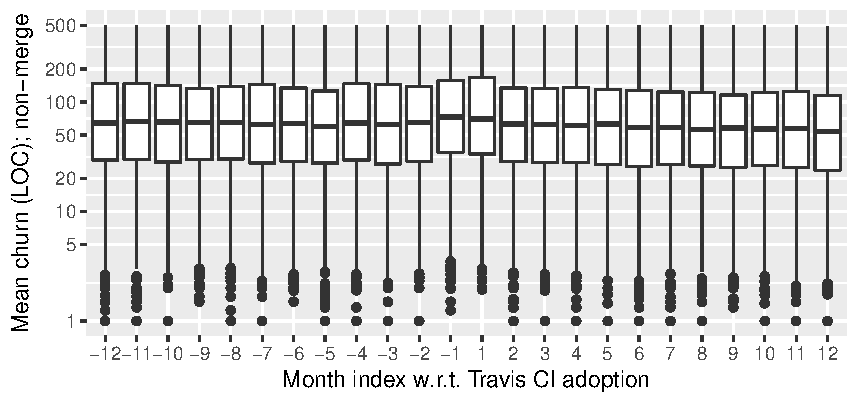
\includegraphics[width=\columnwidth, clip=true, trim=0 0 0 0]{figures/churn.pdf}
\caption{Mean code churn per commit per project, before and after \Tvi.}
\label{fig:churn}
\end{figure}

\smallskip\noindent \emph{Exploratory Study}: 
Figure~\ref{fig:churn} shows boxplots of per-project per-commit mean code 
churn (medians behave similarly) for each of twelve consecutive 30-day time 
intervals before, and after, the \Tvis adoption.
Recall that due to instability, we omit the 30-day time interval centered 
around $t = 0$, when the earliest commit to the \Tvi configuration file, which 
signals adoption, was recorded (Figure~\ref{fig:timeseries}).
The horizontal line in each boxplot is the median value over all projects.

We observe that, pre-\Tvi, the medians are quite stable, dancing around 65 
lines of code churn per commit on average, with large variance.
The 30-day interval just before \Tvis adoption (-1) seems to stand out and is 
slightly higher than the rest (median = 73 LOC), as is the 30-day interval just after 
\Tvi (1).
On the other side, following \Tvis adoption, there seems to be a slight downward 
trend in the medians, which drop to about 53 lines of code churn per commit on 
average in the last period (12).
However, we note the large variance around the medians.

In conclusion, discounting the peak behavior in code churn around adoption 
time, we observe a small reduction in the amounts of code churn from before 
to after the adoption.

%To explore general trends over 
%time, we first look at code churn in months leading up to CI adoption.
%The horizontal line in each boxplot is the median value of all per-project medians, 
%and the black dot is their average value.
%We observe that, for most part, the medians dance around 10 and 12 lines of 
%code churn per period, and the averages between 16 and 18 lines, with large 
%variance and no obvious trend. 
%The 30-day interval just before CI adoption seems to stand out and is higher 
%than the rest.

%Next, we look to the other side of the adoption point. 
%Fig.~\ref{Fig:CodeChurnAfter} shows a boxplot of per-project median code 
%churn for each of nine consecutive 30-day time intervals following CI adoption.
%Here, there seems to be a slight downward trend in both the medians and 
%averages; the former drop monotonically from 13 down to 8 lines of code and 
%the latter down to 15 lines of code.
%However, we note the large variance around the medians.

%The 30- and 60-day intervals just after the adoption point seem to be higher 
%than the rest, and together with the 30-day interval just before adoption of CI 
%seem to form a peak of increased code churn.
%In conclusion, discounting the peak behavior in code churn around CI adoption 
%time, we observe a small reduction in the amounts of code churn from before 
%to after CI adoption.

%% !TEX root = ../CI_Adoption.tex

\begin{table}[t] \centering
\small
  \caption{Model Coefficients for 566 Models of Code Churn}
  \label{Table:rddmodels}
\begin{tabular}{ l  r r r r }        
\hline 

 & $\beta$ & $\gamma$ & $\delta$ & $\beta + \delta$ \\ 
 \hline 
 \hline
not signif. & 504 & 508 & 514 & \\
\hline
signif., $>0$ & 45 & 28 & 10 & 13 \\
\hline
signif., $<0$ & 17 & 30 & 42 & 39 \\
\hline
\end{tabular}
\end{table}

 

\begin{table}[t]
\centering \footnotesize
\rowcolors{3}{Gray}{}
\begin{tabular}{l D{)}{)}{13)3}@{} D{.}{.}{5.5} }
\hline
                                               & \multicolumn{1}{c}{Coeffs (Errors)} & \multicolumn{1}{c}{Sum Sq.} \\
\hline
(Intercept)                            & 1.311 \; (0.132)^{***} & \\
log(TotalCommits)                      & 0.439 \; (0.016)^{***}  & 588.51^{***} \\
AgeAtTravis                            & -0.003 \; (0.000)^{***} & 48.10^{***} \\
log(NumAuthors)                        & -0.173 \; (0.012)^{***} & 158.77^{***} \\
time                                   & 0.002 \; (0.002)       & 0.93 \\ 
interventionTRUE                       & 0.039 \; (0.019)^{*}    & 3.22^{*} \\
time\_after\_intervention              & -0.023 \; (0.002)^{***} & 75.59^{***} \\
%
%
%(Intercept)                                & 1.125 \; (0.161)^{***}  &  \\
%log(TotalCommits)                          & 0.514 \; (0.020)^{***}  & 588.51^{***} \\
%AgeAtTravis                                & -0.003 \; (0.001)^{***} & 48.10^{***} \\
%log(NumAuthors)                            & -0.218 \; (0.016)^{***} & 158.77^{***} \\
%time                                       & 0.002 \; (0.002)       & 0.93 \\
%interventionTRUE                           & 0.072 \; (0.028)^{**}  & 3.22^{*} \\
%time\_after\_intervention                  & -0.024 \; (0.003)^{***} & 75.59^{***} \\
%(Intercept)                                          & 0.069 \; (0.012)^{***}   & \\
%GlobalTime                                    & -0.037 \; (0.005)^{***}  & 15.71^{***} \\
%Projects                                      & 0.263 \; (0.006)^{***}   & 2566.87^{***} \\
%Languages                                     & 0.549 \; (0.004)^{***}   & 11505.20^{***} \\
%$S_\text{Focus}$                                  & -0.300 \; (0.004)^{***}  & 2757.75^{***} \\
%$S_\text{Language}$                               & -0.231 \; (0.003)^{***}  & 2354.39^{***} \\
%AvgProjectsPerDay                             & 0.046 \; (0.004)^{***}   & 215.29^{***} \\
%$S_\text{Switch}$                          & 0.225 \; (0.004)^{***}   & 2255.09^{***} \\
%Projects:$S_\text{Focus}$                  & 0.032 \; (0.003)^{***}   & 0.16^{***} \\
%Languages:$S_\text{Language}$              & -0.045 \; (0.002)^{***}  & 345.96^{***} \\
%Projects:$S_\text{Language}$               & -0.021 \; (0.003)^{***}  & 68.66^{***} \\
%Projects:AvgProjectsPerDay             & -0.024 \; (0.003)^{***}  & 128.60^{***} \\
%$S_\text{Language}$:AvgProjectsPerDay      & 0.026 \; (0.003)^{***}   & 59.86^{***} \\
%Projects:$S_\text{Switch}$          & -0.104 \; (0.003)^{***}  & 404.80^{***} \\
%AvgProjectsPerDay:$S_\text{Switch}$ & 0.058 \; (0.003)^{***}   & 203.12^{***} \\
%$S_\text{Language}$:$S_\text{Switch}$   & -0.029 \; (0.003)^{***}  & 35.99^{***} \\
\hline
%\multicolumn{3}{c}{AIC = 175178.307; BIC =  175303.204; LogLik = -87575.153           }                                          \\
%\rowcolor{white}
%\rowcolor{white}
%\multicolumn{3}{c}{Num. obs. = 55340; Num. groups: Repo = 2405; Language = 22}\\
%AIC                                        & 175178.307              \\
%BIC                                        & 175303.204              \\
%Log Likelihood                             & -87575.153              \\
%Num. obs.                                  & 55340                   \\
%Num. groups: Repo                          & 2405                    \\
%Num. groups: Language                      & 22                      \\
%Var: Repo (Intercept)                      & 0.666                   \\
%Var: Repo interventionTRUE                 & 0.262                   \\
%Cov: Repo (Intercept) interventionTRUE     & -0.138                  \\
%Var: Language (Intercept)                  & 0.145                   \\
%Var: Language interventionTRUE             & 0.003                   \\
%Cov: Language (Intercept) interventionTRUE & 0.002                   \\
%Var: Residual                              & 1.200                   \\
%Analysis of Variance Table of type III  with  Satterthwaite 
%approximation for degrees of freedom
%                        Sum Sq Mean Sq NumDF DenDF F.value    Pr(>F)    
%log(TotalCommits)       760.54  760.54     1  2412  634.04 < 2.2e-16 ***
%AgeAtTravis              49.73   49.73     1  2386   41.46 1.449e-10 ***
%log(NumAuthors)         234.13  234.13     1  2373  195.19 < 2.2e-16 ***
%time                      0.77    0.77     1 50696    0.65   0.42188    
%intervention              8.29    8.29     1    11    6.91   0.02413 *  
%time_after_intervention  95.91   95.91     1 50681   79.96 < 2.2e-16 ***
%---
%Signif. codes:  0 �***� 0.001 �**� 0.01 �*� 0.05 �.� 0.1 � � 1
\hline
\rowcolor{white}
\multicolumn{2}{l}{\scriptsize{$^{***}p<0.001$, $^{**}p<0.01$, $^*p<0.05$}}
\end{tabular}
\caption{Commit churn model. The response is \textbf{log(mean commit churn)}
per month. $R^2_m = 0.1$. $R^2_c = 0.46$.}
\label{table:churn}
 
\end{table}



\smallskip\noindent \emph{Statistical Modeling Study}: 
Guided by our exploratory observations above, we proceed to quantify the 
trends we observed using a mixed-effects RDD model, as described before.
Recall that we modeled a random intercept for \emph{programming language}, 
to allow for language-to-language variability in the response (\ie code in some 
languages being naturally more verbose than in others), and a random 
\emph{intervention} slope and intercept for \emph{project}, to allow for 
project-to-project variability in the response, and the possibility that, on average, 
projects with lower initial churn values may be less strongly affected by adopting 
\Tvis, since their commits are already ``small enough'' for efficient CI.
Recall also that the coefficient for \emph{time} is the slope before adoption,
the coefficient for \emph{intervention} is the size of the effect of CI introduction,
the coefficient for \emph{time\_after\_intervention} is the divergence in the slopes
before and after \Tvis adoption, and the sum of the coefficients for \emph{time}
and \emph{time\_after\_intervention} is the slope of the linear trend after \Tvis
adoption.

Table~\ref{table:churn} summarizes the model.
In addition to the model coefficients and corresponding standard errors, the table 
shows the sum of squares, a measure of variance explained, for each variable.
The statistical significance is indicated by stars.
First, we observe that only the combined fixed-and-random effects model fits the 
data well ($R_c^2 = 0.46$ compared to $R_m^2 = 0.1$), \ie most of the explained 
variability in the data is attributed to project-to-project and language-to-language
variability, rather than any of the fixed effects, either controls or RDD-related.

Next, we turn to our controls and main predictors.
The controls behave unsurprisingly.
Overall bigger projects (\emph{TotalCommits}) tend to churn more, other things
held constant; older projects (\emph{AgeAtTravis}) tend to churn less, perhaps 
as they have reached maturity and a more stationary stage in their evolution;
projects with a larger contributor base (\emph{NumAuthors}) also tend to churn
less, which is in line with the expectation that occasional contributors to open 
source projects are generally less active than core developers.

After controlling for confounds, we move on to the main predictors. 
We observe that the coefficient for \emph{time} is not statistically significant, 
\ie there is no baseline trend in commit churn before CI adoption, and the 
\emph{intervention}, although statistically significant, has a small effect.
However, \emph{time\_after\_intervention} has a statistically significant, 
negative coefficient, with a notable effect size.
Taken together, this confirms a decreasing trend in commit churn after 
adopting \Tvis.

\smallskip\noindent \emph{Discussion}:
Across our large sample (2,401 projects across 22 programming languages),
our modeling study revealed a statistically significant, but small, discontinuity
in the commit churn time series when adopting \Tvis; and a statistically 
significant decreasing linear trend with time in code churn, after adopting \Tvis.
The former is not unexpected, as one can reasonably expect that more 
maintenance work may be going on in preparation for the transition to \Tvis, 
and that the projects go through some adjustment/cleanup period right after.
The increased code churn on both sides near the CI adoption time is also
indication of this, as are the survey results.  
Indeed, when asked about the introduction of \Tvis, respondents frequently refer to 
test automation being introduced around the same time as \Tvi ``as contributors 
couldn't be trusted to run test suite on their own'' (R25). Furthermore, respondents 
indicate that \Tvi has been introduced as ``a part of automated package/release effort'' (R38) 
and to ``deploy artifacts to S3 on each commit, as part of our deployment process using 
Amazon CodeDeploy'' (R34).

The latter is consistent with Fowler's recommended good practices of CI, of 
committing smaller changes to the code.
The expected decrease in the size of the commits is echoed by one of the 
survey respondents: ``commits became smaller and more frequent, to check 
the build; pull requests became easier to check'' (R4).
However, the decreasing trend we observed is not steep.
Survey responses provide a possible explanation: several developers 
referred to pull request integration as the reason for introducing \Tvis, and 
while R31 and R50 state that \Tvis is used both for commits and for pull 
requests, R11, R21, and R37 explicitly state that \Tvis is applied solely to 
pull requests, \ie in those projects push commits are outside the scope of \Tvis.
In other words, if in a project not all commits are subjected to \Tvis, then 
there may be less incentive to follow Fowler's recommended good practices 
related to commit churn.

At the same time, a different respondent indicated that \Tvis discourages 
him/her from making trivial commits (R11), suggesting instead that the 
commits he/she makes are likely to be larger;
therefore, our global decreasing trend may be weakened by local trends
in the opposite direction.
Our model found evidence for strong project-specific effects: 
project-to-project and language-to-language differences, as captured by 
our random effects, better explain the overall data variability. 
This suggests that any phenomena giving rise to pressures to increase 
or reduce code churn are perhaps subordinate in magnitude to other, 
more pressing phenomena of local, \ie project-specific, character.

Alternatively, the decreasing trend in commit churn is also consistent with 
the observation by Brindescu \etal~\cite{brindescu2014centralized} that, 
as projects age, bug-fixing commits, which on average are smaller, 
become more prevalent than commits adding new features, which on 
average are larger.

\as{Say something about SE practice/research implications}
Our results suggest that while the Fowler's good practice of small commits is followed to some extent but the project-to-project and language-to-language differences are more important and might overshadow the overall trend.
\as{Still thinking} 


%Most of the projects did not show linear trends with time in code churn, on 
%either side of the CI adoption time.
%One explanation consistent with this is that any phenomena giving rise to 
%pressures to increase or reduce code churn are not long term/sustained or, 
%alternatively, perhaps they are subordinate in magnitude to other, more 
%pressing phenomena of local character in time.
%It is also likely that our models and data are insufficient to capture them.
%Some of the reasons for this are: low temporal resolution, high dispersion 
%of the data, non-uniform distribution of the events across time, and project 
%specific considerations that we could not model.

%Our exploratory study showed a peak around CI adoption time and a slight 
%downward trend following CI adoption.
%The modeling study showed that when linear trends were present (in 15\% 
%of the models), the downward one after CI adoption were twice as frequent 
%as the upward one, a reversal of the pattern in the trends from before CI.
%This is consistent with Fowler's recommended good practices of CI, of 
%committing smaller changes to the code.
%Alternatively, it is also consistent with the observation by Brindescu 
%\etal~\cite{brindescu2014centralized} that, as projects age, bug-fixing 
%commits, which on average are smaller, become more prevalent than 
%commits adding new features, which on average are larger.

%The models also showed that when present, the effect of CI adoption on the 
%amount of code churn right after was positive in more cases than negative.
%The increased code churn on both sides near the CI adoption time is 
%arguably in line with expectations that more maintenance work may be 
%going on in preparation for the transition to CI, and that the projects go 
%through some adjustment/cleanup period right after.



%The model fits the data well; it explains 35% of the variability in the data using only the fixed effects (Rm2 = 0.35), and 55% when considering both the fixed and random effects (Rc2 = 0.55).

%deviations in intercept and slope of that subject�s time trend from the population values.
%(1 + Days | Subject)
%we allow for the possibility that, for example, subjects with higher initial reaction times may, on average, be more strongly affected by sleep deprivation.

%For each project, we fitted a sharp RDD model, as described before.
%Recall that because of the peak we observed, we eliminated the time point 
%immediately before and the one immediately after the CI adoption time, so as 
%they do not throw off the regression models.
%Table~\ref{Table:rddmodels} summarizes the results for the models on the 
%remaining 16 time points.
%Recall that $\beta$ is the slope before, $\gamma$ the size of the effect of 
%CI introduction, $\delta$ is the divergence in the slopes before and after CI 
%adoption, and $\beta + \delta$ the slope of the linear trend after CI adoption.

%Of the 567 models, in 487 there was no significant linear relationship of 
%code churn to time, \ie there was no linear trend.
%In 47 projects there was a rising trend before CI and in 33 projects a falling 
%trend before CI.
%Similarly, in 507 projects no effect of CI introduction on code churn was found. 
%Among the 58 projects where an effect was significant, in 34 the trend was 
%positive, \ie code churn increased, and in 24 it was negative, \ie code churn 
%decreased.
%Interestingly, while in 487 projects no change of slope in the trends before 
%and after CI adoption was found, in the 80 projects with significant change 
%of trends, a reduction in the slope was more prevalent than an increase by 
%about 2 to 1.
%This carried over into trends following CI adoption: out of the 80 significant 
%trend changes, 55 are downward trends, and only 25 are upward.


%Table XX: Projects with statistical negative trends after CI


\bv{I'm here}

\begin{figure}[t]
\centering
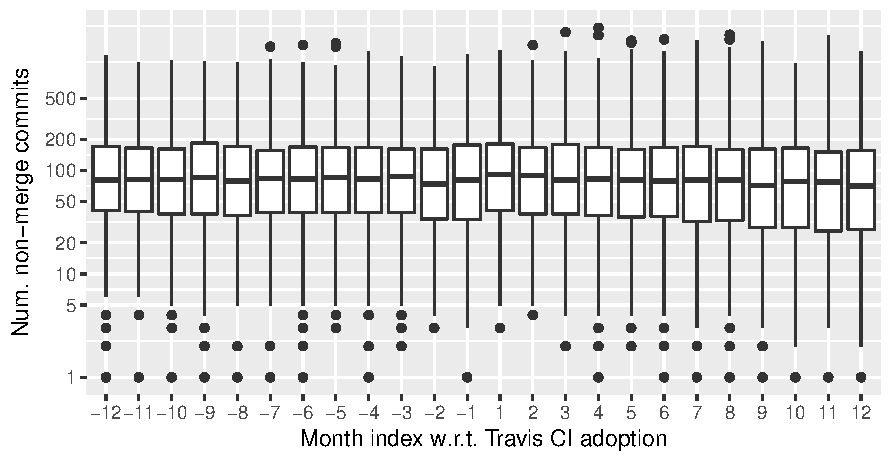
\includegraphics[width=\columnwidth, clip=true, trim=0 0 0 0]{figures/freq-non-merge.pdf}
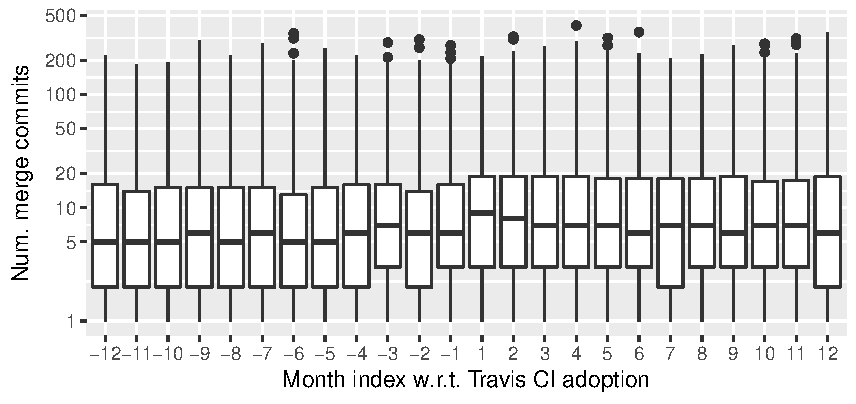
\includegraphics[width=\columnwidth, clip=true, trim=0 0 0 0]{figures/freq-merge.pdf}
\caption{Evolution of mean code churn before and after the \Tvis adoption.}
\label{fig:freq}
\end{figure}

\begin{figure}[t]
\centering
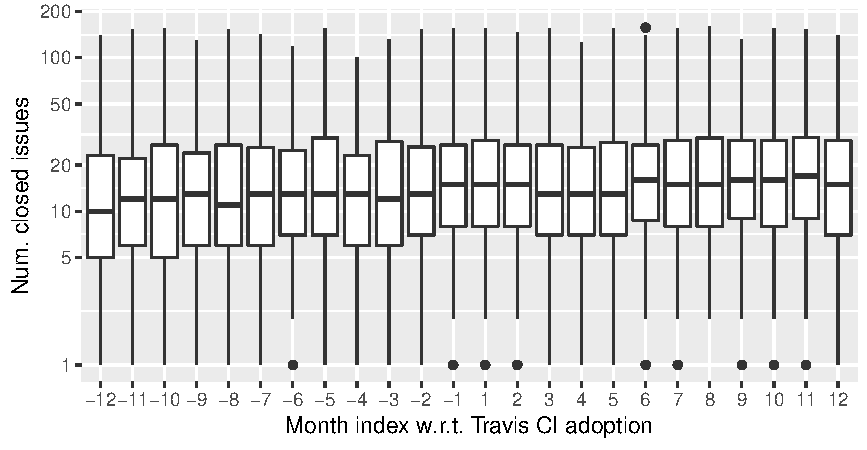
\includegraphics[width=\columnwidth, clip=true, trim=0 0 0 0]{figures/issues.pdf}
\caption{Evolution of the number of closed issues before and after the \Tvis adoption.}
\label{fig:issues}
\end{figure}

\begin{figure}[t]
\centering
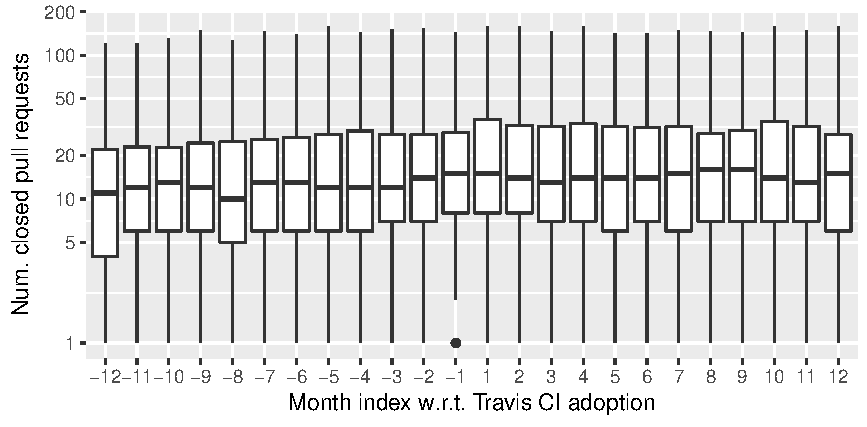
\includegraphics[width=\columnwidth, clip=true, trim=0 0 0 0]{figures/prs-full.pdf}
\caption{Evolution of the number of closed pull requests before and after the \Tvis adoption.}
\label{fig:prs}
\end{figure}


\begin{figure}[t]
\centering
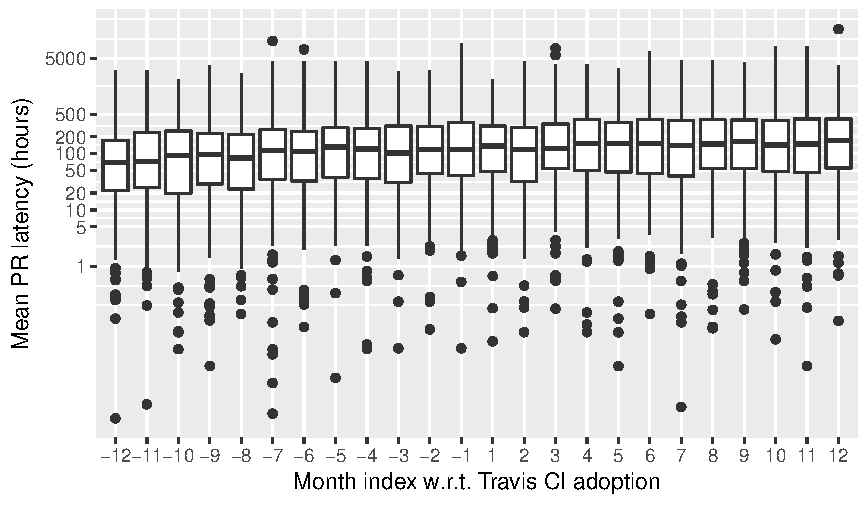
\includegraphics[width=\columnwidth, clip=true, trim=0 0 0 0]{figures/pr-latency-mean.pdf}
\caption{Evolution of the mean PR latency before and after the \Tvis adoption.}
\label{fig:pr-latency}
\end{figure}



 

\begin{table}[t]
\caption{Commit frequency model. The response is \textbf{log(number of non-merge commits)}
per month. $R^2_m = 0.57$. $R^2_c = 0.77$.}
\label{table:freq} 
\centering \footnotesize
\rowcolors{3}{Gray}{}
\begin{tabular}{l D{)}{)}{13)3}@{} D{.}{.}{5.5} }
\hline
                                               & \multicolumn{1}{c}{Coeffs (Errors)} & \multicolumn{1}{c}{Sum Sq.} \\
\hline
(Intercept)                            & -1.660 \; (0.102)^{***} & \\
log(TotalCommits)                      & 0.662 \; (0.015)^{***} & 933.1^{***}  \\
log(num\_merge\_commits+1)           & 0.558 \; (0.004)^{***} & 8323.6^{***} \\
AgeAtTravis                            & -0.003 \; (0.000)^{***} & 30.7^{***}\\
log(NumAuthors)                        & -0.215 \; (0.011)^{***} & 173.2^{***}\\
time                                   & -0.012 \; (0.001)^{***} & 40.8^{***}\\
interventionTRUE                       & 0.102 \; (0.018)^{***} & 15.1^{***} \\
time\_after\_intervention              & -0.013 \; (0.002)^{***} & 25.5^{***}\\
\hline
%AIC                                    & 111917.158              \\
%BIC                                    & 112031.638              \\
%Log Likelihood                         & -55945.579              \\
%Num. obs.                              & 49323                   \\
%Num. groups: Repo                      & 2401                    \\
%Num. groups: Language                  & 22                      \\
%Var: Repo (Intercept)                  & 0.399                   \\
%Var: Repo interventionTRUE             & 0.339                   \\
%Cov: Repo (Intercept) interventionTRUE & -0.178                  \\
%Var: Language (Intercept)              & 0.010                   \\
%Var: Residual                          & 0.462                   \\
\hline
\rowcolor{white}
\multicolumn{2}{l}{\scriptsize{$^{***}p<0.001$, $^{**}p<0.01$, $^*p<0.05$}}
\end{tabular}
\end{table}



 

\begin{table}[t]
\centering \footnotesize
\rowcolors{3}{Gray}{}
\begin{tabular}{l D{)}{)}{13)3}@{} D{.}{.}{5.5} }
\hline
                                               & \multicolumn{1}{c}{Coeffs (Errors)} & \multicolumn{1}{c}{Sum Sq.} \\
\hline
(Intercept)                            & -1.680 \; (0.364)^{***} & \\
log(TotalCommits)                      & 0.443 \; (0.049)^{***} & 42.54^{***}  \\
AgeAtTravis                            & -0.006 \; (0.001)^{***} & 8.83^{***}\\
log(NumAuthors)                        & 0.119 \; (0.039)^{**}   & 4.72^{**}\\
time                                   & 0.021 \; (0.004)^{***}  & 16.00^{***}\\
interventionTRUE                       & 0.030 \; (0.049)         0.19&\\
time\_after\_intervention              & -0.019 \; (0.005)^{***}  &  5.99^{***}\\
\hline
%AIC                                    & 13679.398               \\
%BIC                                    & 13759.398               \\
%Log Likelihood                         & -6827.699               \\
%Num. obs.                              & 5806                    \\
%Num. groups: Repo                      & 280                     \\
%Num. groups: Language                  & 20                      \\
%Var: Repo (Intercept)                  & 0.403                   \\
%Var: Repo interventionTRUE             & 0.213                   \\
%Cov: Repo (Intercept) interventionTRUE & -0.134                  \\
%Var: Language (Intercept)              & 0.019                   \\
%Var: Residual                          & 0.513                   \\
%
%(Intercept)                            & -2.540 \; (0.180)^{***} & \\
%log(TotalCommits)                      & 0.396 \; (0.025)^{***} & 155.91^{***} \\
%AgeAtTravis                            & -0.006 \; (0.001)^{***} & 47.72^{***}\\
%log(NumAuthors)                        & 0.224 \; (0.019)^{***} & 83.73^{***} \\
%time                                   & 0.012 \; (0.002)^{***} & 13.58^{***} \\
%interventionTRUE                       & 0.049 \; (0.028)       & 2.02 \\
%time\_after\_intervention              & -0.008 \; (0.003)^{*}  & 3.77^{*} \\
%\hline
%AIC                                    & 58524.762               \\
%BIC                                    & 58620.964               \\
%Log Likelihood                         & -29250.381              \\
%Num. obs.                              & 22401                   \\
%Num. groups: Repo                      & 1716                    \\
%Num. groups: Language                  & 22                      \\
%Var: Repo (Intercept)                  & 0.641                   \\
%Var: Repo interventionTRUE             & 0.301                   \\
%Cov: Repo (Intercept) interventionTRUE & -0.159                  \\
%Var: Language (Intercept)              & 0.050                   \\
%Var: Residual                          & 0.627                   \\
\hline
\rowcolor{white}
\multicolumn{2}{l}{\scriptsize{$^{***}p<0.001$, $^{**}p<0.01$, $^*p<0.05$}}
\end{tabular}
\caption{Issues model. The response is \textbf{log(number of issues closed)}
per month. $R^2_m = 0.17$. $R^2_c = 0.53$.}
\label{table:issues}
 
\end{table}



 

\begin{table}[t]
\caption{Pull request latency model. The response is \textbf{log(mean pull request latency)}
per month, in hours. $R^2_m = 0.05$. $R^2_c = 0.31$.}
\label{table:latency}
\centering \footnotesize
\rowcolors{3}{Gray}{}
\begin{tabular}{l D{)}{)}{13)3}@{} D{.}{.}{5.5} }
\hline
                                               & \multicolumn{1}{c}{Coeffs (Errors)} & \multicolumn{1}{c}{Sum Sq.} \\
\hline
(Intercept)                            & 0.052 \; (0.519)      & \\
log(TotalCommits)                      & 0.157 \; (0.068)^{*} & 7.89^{*}   \\
AgeAtTravis                            & -0.002 \; (0.002)    & 1.00  \\
log(NumAuthors)                        & 0.225 \; (0.062)^{***} & 19.72^{***}\\
time                                   & 0.030 \; (0.012)^{*}  & 8.60^{*} \\
interventionTRUE                       & -0.160 \; (0.153)    & 1.65  \\
time\_after\_intervention              & -0.022 \; (0.019)    & 2.03  \\
\hline
%Analysis of Variance Table of type III  with  Satterthwaite 
%approximation for degrees of freedom
%                         Sum Sq Mean Sq NumDF   DenDF F.value    Pr(>F)    
%log(TotalCommits)        7.8943  7.8943     1  200.00  5.2679 0.0227593 *  
%AgeAtTravis              1.0013  1.0013     1  194.21  0.6682 0.4146849    
%log(NumAuthors)         19.7179 19.7179     1  197.77 13.1579 0.0003644 ***
%time                     8.6001  8.6001     1 1475.42  5.7389 0.0167173 *  
%intervention             1.6486  1.6486     1  886.22  1.1001 0.2945248    
%time_after_intervention  2.0330  2.0330     1 1506.63  1.3566 0.2443056    

%AIC                                    & 5558.908               \\
%BIC                                    & 5623.561               \\
%Log Likelihood                         & -2767.454              \\
%Num. obs.                              & 1616                   \\
%Num. groups: Repo                      & 203                    \\
%Num. groups: Language                  & 7                      \\
%Var: Repo (Intercept)                  & 0.638                  \\
%Var: Repo interventionTRUE             & 0.478                  \\
%Cov: Repo (Intercept) interventionTRUE & -0.342                 \\
%Var: Language (Intercept)              & 0.000                  \\
%Var: Residual                          & 1.499                  \\
%
%(Intercept)                            & 2.510 \; (0.526)^{***} & \\
%log(TotalCommits)                      & -0.138 \; (0.073)    & 6.79 \\
%AgeAtTravis                            & 0.007 \; (0.002)^{***} &  24.44^{***} \\
%log(NumAuthors)                        & 0.474 \; (0.064)^{***} &  101.27^{***} \\
%time                                   & 0.055 \; (0.007)^{***} &  113.44^{***} \\
%interventionTRUE                       & -0.103 \; (0.082)     &  2.95 \\
%time\_after\_intervention              & -0.032 \; (0.010)^{**} &  19.09^{**} \\
%\hline
%AIC                                    & 23087.126              \\
%BIC                                    & 23168.260              \\
%Log Likelihood                         & -11531.563             \\
%Num. obs.                              & 6382                   \\
%Num. groups: Repo                      & 306                    \\
%Num. groups: Language                  & 21                     \\
%Var: Repo (Intercept)                  & 1.085                  \\
%Var: Repo interventionTRUE             & 0.392                  \\
%Cov: Repo (Intercept) interventionTRUE & -0.275                 \\
%Var: Language (Intercept)              & 0.058                  \\
%Var: Residual                          & 1.870                  \\
\hline
\rowcolor{white}
\multicolumn{2}{l}{\scriptsize{$^{***}p<0.001$, $^{**}p<0.01$, $^*p<0.05$}}
\end{tabular} \vspace{-0.4cm}
\end{table}




\begin{figure}[t]
\centering
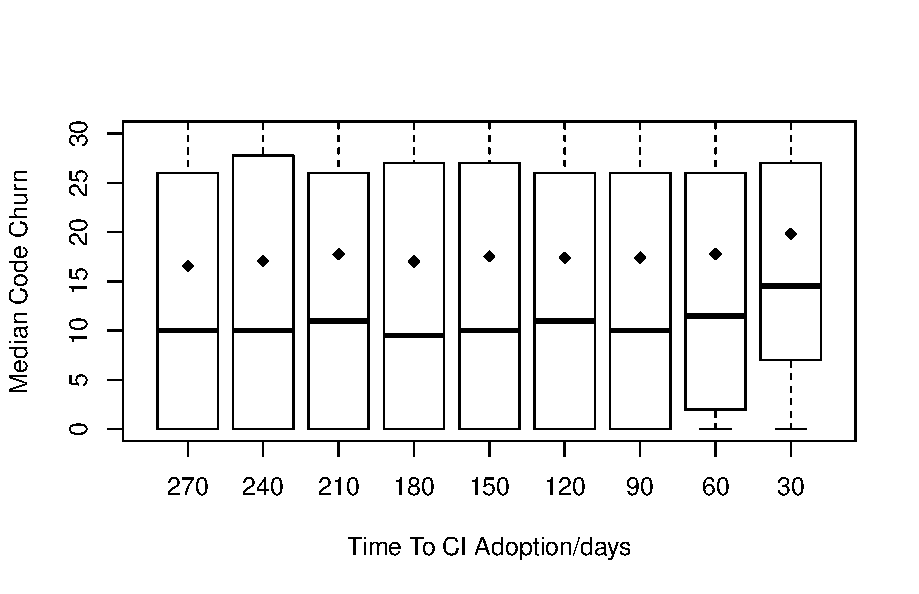
\includegraphics[width=0.45\textwidth, clip=true, trim=0 15 15 50]{churn_before.pdf}
\caption{Code churn before \Tvis adoption.}
\label{Fig:CodeChurnBefore}\vspace{-0.3cm}
\end{figure}


\begin{figure}[t]
\centering
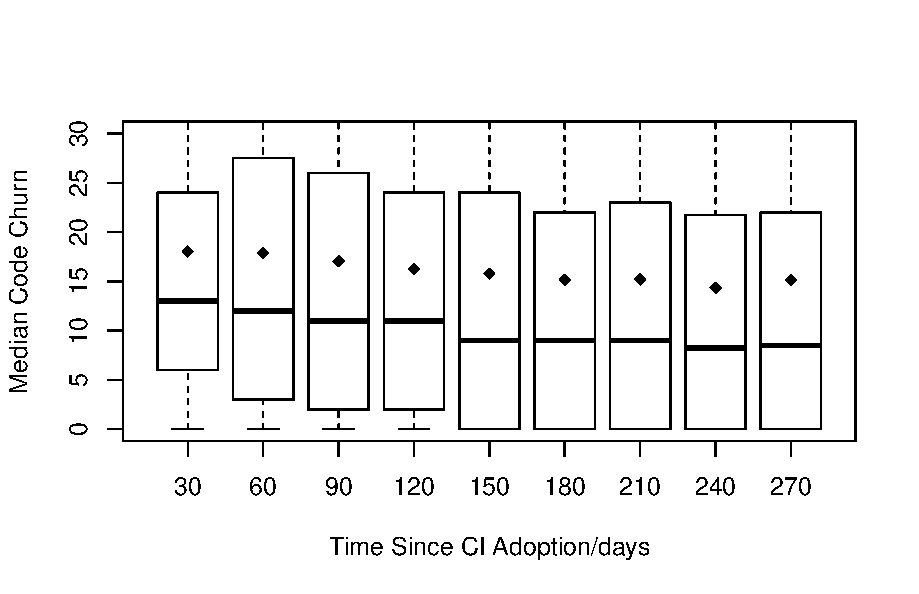
\includegraphics[width=0.45\textwidth, clip=true, trim=0 15 15 50]{churn_after.pdf}
\caption{Code churn after \Tvis adoption.}
\label{Fig:CodeChurnAfter}\vspace{-0.3cm}
\end{figure}



\subsection{RQ2: Trends in Commit Frequency}

The second practice we examine is commit frequency.
We examine this question from two directions by looking separately at the non-merge commits at the merge commits. 
%(we obtained the latter as described previously in the Methods section).

We started from the same data as before, 567 projects, each with at least 500 
non-merge commits.
Additionally, we restricted the projects for the  merge commits study so that we only look at projects that have at least 20 merge commits over the 18 time points, \ie on average about 1 per time point.
This filtering yielded a set of 370 projects for the merge commit frequency study.

\begin{figure}[!t]
\centering
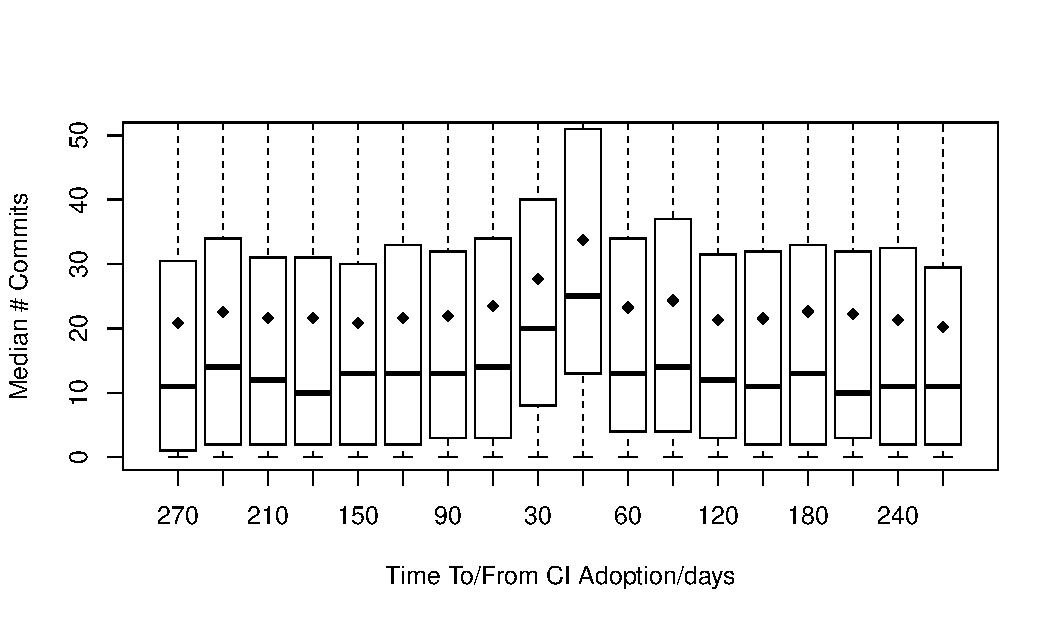
\includegraphics[width=0.45\textwidth, clip=true, trim=0 15 15 50]{numbercommits.pdf}
\caption{Non-merge commit frequency before and after CI adoption}
\label{Fig:NumberCommits}
\end{figure}

\begin{figure}[!t]
\centering
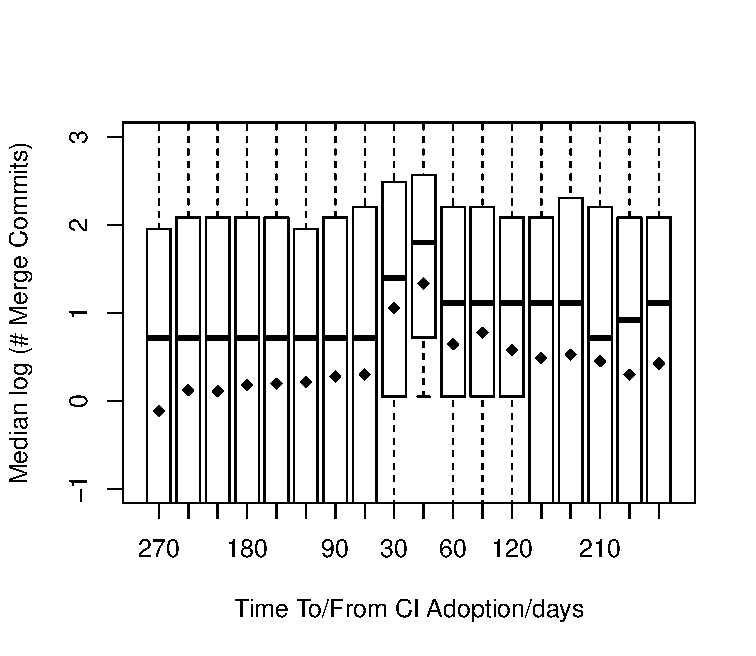
\includegraphics[width=0.45\textwidth, height=1.5in, clip=true, trim=0 15 15 50]{merges.pdf}
\caption{Merge commit frequency before and after CI adoption}
\label{Fig:MergeCommits}
\end{figure}

\smallskip\noindent \emph{Exploratory Study}: 
To explore general trends over time, we first look at commit frequency in 
the months leading up to CI adoption.
Figs.~\ref{Fig:NumberCommits} and \ref{Fig:MergeCommits} show the boxplots of per-project median 
number of non-merge commits, and merge commits, respectively, for each of nine consecutive 30-day time intervals 
before CI adoption and, respectively, nine consecutive 30-day time intervals 
after CI adoption.
We use a log-scale for the merge commits due to the overdispersion of the data which is sparse over the time periods we have chosen.
As before, the horizontal line in each boxplot is the median value of all 
per-project medians, and the black dot is their average value.

As with code churn, here we also see a peak in the 30-day 
interval just before and the one just after CI adoption.
We do not observe an apparent trend in the 
median or average non-merge commit frequency.
We do observe an upward trend in merge commits, but the variance in the data is large.

\smallskip\noindent \emph{Statistical Modeling Study}: 
As in RQ1, we fitted a sharp RDD model for each project, as described before.
Tables~\ref{Table:rddmodels_freq} and ~\ref{Table:rddmodels_merge_freq} summarize the results.
As before, we eliminated one time point on either side of the CI adoption 
time, so that the peaks at those times  do not throw off the regression models.
% !TEX root = ../CI_Adoption.tex

\begin{table}[t] \centering
\small
  \caption{Model Coefficients for 567 Models of Commit Frequency}
  \label{Table:rddmodels_freq}
\begin{tabular}{ l  r r r r }        
\hline 

 & $\beta$ & $\gamma$ & $\delta$ & $\beta + \delta$ \\ 
 \hline 
 \hline
not signif. & 452 & 466 & 454 & \\
\hline
signif., $\ge 0$ & 71 & 59 & 33 & 42 \\
\hline
signif., $<0$ & 44 & 42 & 80 & 71 \\
\hline
\end{tabular}
\end{table}

\begin{table}[t] \centering
\small
  \caption{Model Coefficients for 370 Models of Merge Commit Frequency}
  \label{Table:rddmodels_merge_freq}
\begin{tabular}{ l  r r r r }        
\hline 

 & $\beta$ & $\gamma$ & $\delta$ & $\beta + \delta$ \\ 
 \hline 
 \hline
not signif. & 296 & 307 & 301 & \\
\hline
signif., $\ge 0$ & 46 & 35 & 26 & 44 \\
\hline
signif., $<0$ & 28 & 28 & 43 & 30 \\
\hline
\end{tabular}
\end{table}

For the non-merge commits, in 452 (80\%) of the models, there was no significant linear relationship 
between  frequency and time, \ie there was no linear trend.
In 71 projects there was a rising trend in commit frequency before CI 
and in 44 projects a falling trend before CI.
Similarly, in 466 projects no effect of CI introduction on commit frequency 
was found. 
Among the 101 projects where an effect was significant, in 59 the trend 
was positive, \ie commit frequency increased, and in the rest it was 
negative, \ie commit frequency decreased.
The mean value over all projects for $\gamma$, the effect size of CI 
adoption, was $1.1$ commit.
While in 454 projects no change of slope in the trends before and after CI 
adoption was found, in the 113 with significant change of trends a reduction 
in the slope was more prevalent than an increase by about 2.5 to 1.
This carried over to a lesser degree into trends in commit frequency 
following CI adoption: out of the 113 significant trend changes, 71 are 
downward trends, and 42 are upward.

For merge commits (Table~\ref{Table:rddmodels_merge_freq}), the results 
are qualitatively similar to those for non-merge commits.

\smallskip\noindent \emph{Discussion}:
As was the case for code churn, most projects did not have longitudinal 
linear trends in non-merge commits, for reasons probably similar to those 
in case of code churn.

Even though  we observed a post-CI adoption increase in merge commits 
in our exploratory study, the statistical tests did not confirm that to be the 
case for more than 20\% of the projects. 
We attribute this disparity to the large variance in the data and especially 
the sparsity of merge commits over time. 

While our exploratory study did not suggest presence of a trend, the 
modeling study suggests that right after CI adoption there is a slight 
positive effect in both the merge and non-merge commits (after removing the peak months around CI adoption time). 
However, this effect is not sustained.
% if a linear trend is present, which is 2.5 times as likely to be decreasing as increasing. 

Given the expected increase in the frequency of commits expressed and 
encouraged by Fowler, our results might appear surprising.
It is possible that some saturation to the commit frequency has already 
been reached even before the CI adoption time.
As we see next, it is also likely that instead developers are spending more time on 
automated testing.


%\as{Vladimir, do you have a cross-combination data, such as \# decrease in churn AND increase in frequency?}



\subsection{RQ3: Trends in Issue Report Frequency}

The 3rd practice we examine is issue report frequency.
As above, we use data on 293 projects, each with 
100+ issues.

\begin{figure}[t]
\centering
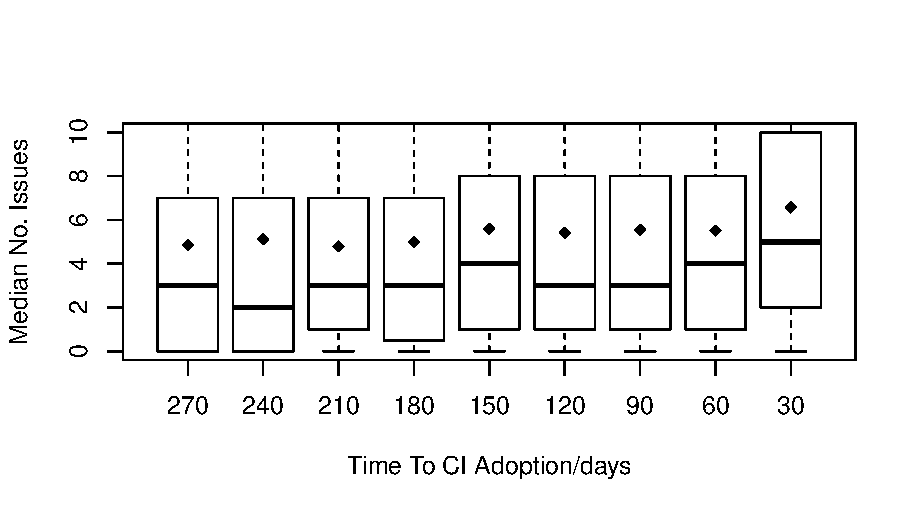
\includegraphics[width=0.45\textwidth, clip=true, trim=0 15 15 50]{issues_before.pdf}
\caption{Median number of issues before CI adoption}
\label{Fig:IssuesBefore}
\end{figure}


\begin{figure}[t]
\centering
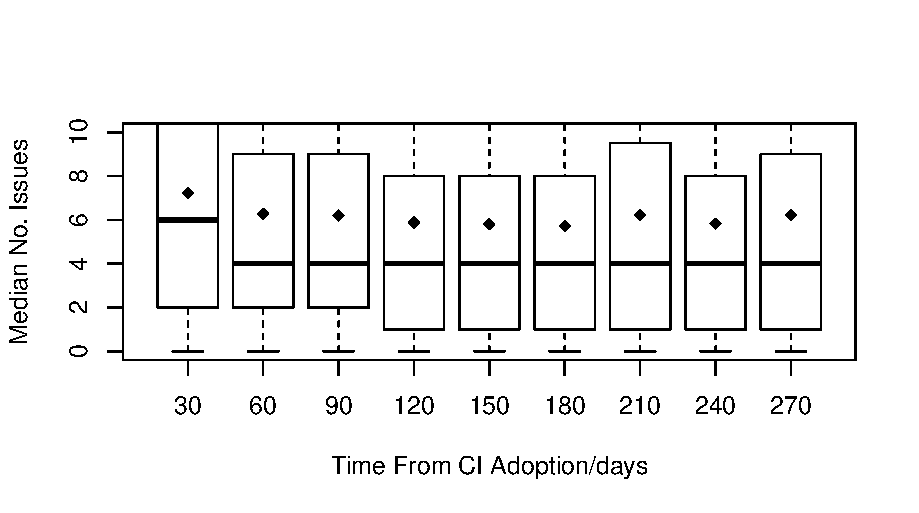
\includegraphics[width=0.45\textwidth, clip=true, trim=0 15 15 50]{issues_after.pdf}
\caption{Median number of issues after CI adoption}
\label{Fig:IssuesAfter}
\end{figure}

\smallskip\noindent \emph{Exploratory Study}:
We follow the same approach as in RQ1 and RQ2 and compare the 
medians and the averages in the number of issues per time period, in the 
months before and after CI adoption.
Fig.~\ref{Fig:IssuesBefore} and \ref{Fig:IssuesAfter} plot the number of 
issues per unit time period.
Observing these figures shows that the months immediately preceding 
and following the adoption of CI exhibit the highest number of issues.
Besides those, before CI adoption the median number of issues per period seem to vary between 2 and 4, with most of them being at 3, while the averages are between 5 and 6.
Following CI adoption the median of the number of issues seems to 
stabilize at 4 per period, and the averages are between 6 and 7.

% !TEX root = ../CI_Adoption.tex

\begin{table}[t] \centering
\small
  \caption{Model Coefficients for 291 Models of Issues Frequency}
  \label{Table:rddmodels_freq}
\begin{tabular}{ l  r r r r }        
\hline 

 & $\beta$ & $\gamma$ & $\delta$ & $\beta + \delta$ \\ 
 \hline 
 \hline
not signif. & 230 & 254 & 242 & \\
\hline
signif., $>0$ & 43 & 26 & 14 & 15 \\
\hline
signif., $<0$ & 18 & 11 & 35 & 33 \\
\hline
\end{tabular}
\end{table}

\smallskip\noindent \emph{Modeling Study}:
Results of the RDD modeling are summarized in Table~\ref{Table:rddmodels_issues}.
The time period before and the one after the time of CI adoption have been removed from the modeling, as explained in RQ1 above.
The lower number of projects in Table~\ref{Table:rddmodels_issues} 
compared to Tables~\ref{Table:rddmodels} and~\ref{Table:rddmodels_freq} 
should not be surprising. 
Recall from Section~\ref{sec:dd} that to answer RQ3 we have focused on 
projects having at least 100 issues, further reducing the size of the data set 
used in RQ1 and RQ2 to 293.
We have fitted models to 291 projects of the 293, however in most cases we 
did not observe linear trends.
When a linear trend has been observed than it was more than twice more 
often decreasing than increasing.
The mean value over all projects for $\gamma$, the effect size of CI adoption, 
was $1.0$ issue.


\smallskip\noindent \emph{Discussion}:
Again, most of the projects did not have longitudinal linear trends for reasons probably similar to those in the case of the code churn.

As in RQ1, our exploratory study showed a peak in the median number of issues per period around CI adoption time, and an upward trend following CI adoption.
The modeling study showed that when linear trends were present (in 20\% 
of the models), the downward one after CI adoption were 2.5 times as frequent 
as the upward one, a reversal of the pattern in the trends from before CI.
This has to be considered in combination with the size of the effect of CI adoption, which is $1$ issue per period additional.
Thus, the number of issues increases significantly overall after CI adoption, to the tune of $33\%$, and then has a pressure of slight reduction over time.

This is consistent with an increased number of issues brought up after CI adoption. Some of those are invariably related to the change in the way things are done, and the transition. Others may be related to the increased automated testing which likely discovers more concerns and bugs, which are then mentioned in issues.
Overall, this result shows that the adoption of CI brings about more issues, as expected.

\as{Survey}
Survey participants experience \Tvi as beneficial for bug detection: ``I think we produce less bugs'' (R45), ``there was an immediately noticeable improvement in terms of the number of serious bugs in production'' (R51). 
An interesting insight into this matter is provided by R16: while several survey respondents have indicated that \Tvis is not consistent in terms of performance and relatively slow, those performance aspects provided R16 with means to detect ``more flaky issues'' ``which where only visible on \Tvi''. 

\subsection{RQ4: Trends in Testing}

The last development practice we examine is testing and the evolution 
of the types of errors revealed by automated testing.
The data consists of 250 projects, each with at least 100 builds, and 90\% 
of builds executing tests.

\begin{figure}[!t]
\centering
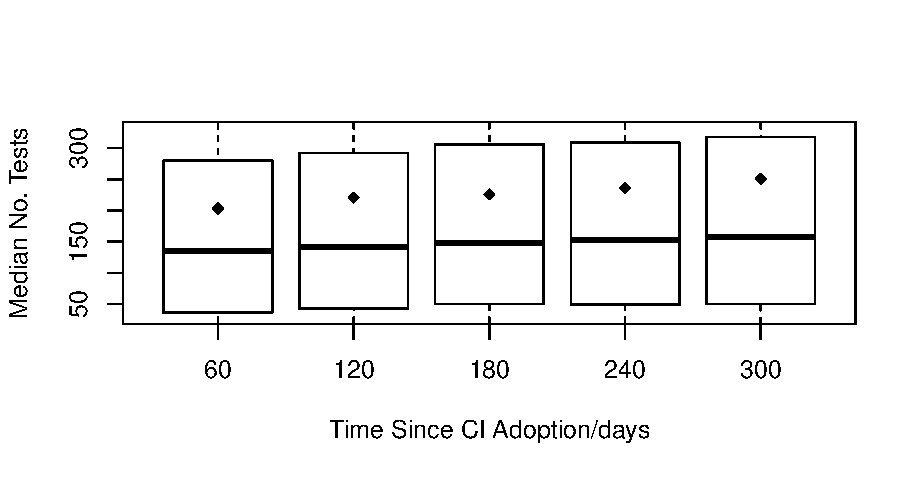
\includegraphics[width=0.45\textwidth, clip=true, trim=0 15 15 50]{tests.pdf}
\caption{Unit tests per build following CI adoption}
\label{Fig:Tests}
\end{figure}

\smallskip\noindent \emph{Exploratory Study}: 
As before, we first look for general trends over time.
Fig.~\ref{Fig:Tests} shows a boxplot of per-project median number of tests 
per build, for each of five consecutive 60-day time intervals before CI adoption.
We aggregated the data here in 60 day intervals to make it easier to visualize 
the trend, since the differences are small.
The horizontal line in each boxplot is the median value of all per-project medians, 
and the black dot is their average value.
We observe a monotonically increasing trend in both the medians, from 140 to 
160 tests per build, and the means, from 205 to 245 tests per build, \ie 15\% to 
20\% increase. 

To ascertain if the complexity of builds increases over time, we also calculated 
the average number of jobs per build.
The median is $1$ for all five time intervals.
These two findings suggest strongly that there is an increase in the number of 
unit tests per build over time.
This, coupled with our finding that builds are not getting more complex over time indicates that developers are likely spending more time on 
automated testing since CI adoption.
This is consistent with Fowler's ``good practices" proposal.



\smallskip\noindent \emph{Error Types Study}:
We also looked at the evolution of the error types in builds over time after CI 
adoption.
For all 250 projects above, we looked at the builds that resulted in errors, 
and deconvolved the errors into 8 types, as described above.
We did this over 3 intervals: 0-60 days, 61-180 days, and 181-300 days (\ie 
corresponding to the first, third, and fifth interval in Fig.~\ref{Fig:Tests}).
The results are shown in Fig.~\ref{Fig:BugTypes}, where on the y-axis are 
the proportion of all erroneous builds that yield that error type.
We find an apparent upward trend over time in most error type categories, 
most notably compile errors, execution errors, failed tests, and skipped 
test.\footnote{The median number of error types per build remained $2$ over 
time.}
All these are consistent with an increase in the amount of code being built 
and tested per build, as well as an increasing management of errors by 
skipping tests, likely to aid in debugging.
On the other hand, we find a decreasing trend among errors related to missing 
files/dependencies, and time-outs, both consistent with those errors being less 
of an issue over time, as developers are acculturating to the CI mediated 
processes.

Thus, overall we find an expected adjustment to the automated testing and 
error handling, with an indication that debugging complexity grows over time.

%%this is the old plots
%\begin{figure}[!t]
%\centering
%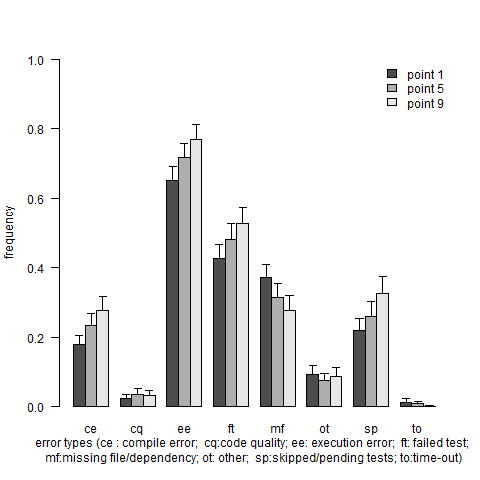
\includegraphics[width=0.45\textwidth, clip=true, trim=0 15 15 50]{plot_together.png}
%\caption{Evolution of Error Types Since CI Adoption}
%\label{Fig:BugTypesold}
%\end{figure}


%this is the new plots
\begin{figure}[!t]
	\centering
	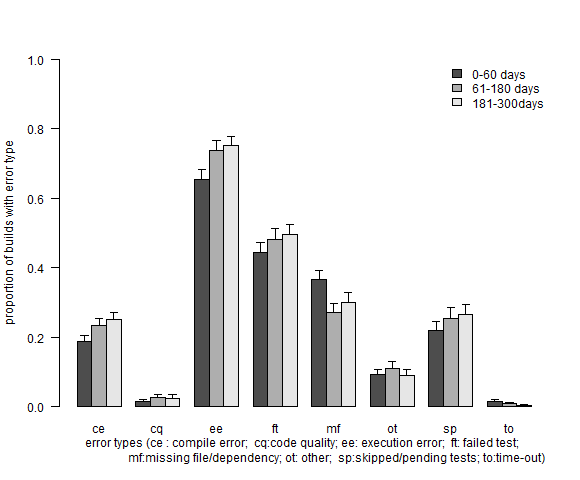
\includegraphics[width=0.45\textwidth, clip=true, trim=0 15 15 50]{new_plot_together.png}
	\caption{Evolution of Error Types Since CI Adoption}
	\label{Fig:BugTypes}
\end{figure}



%% !TEX root = CI_Adoption.tex
\section{Survey}
\label{sec:survey}
To obtain more profound insights in the adoption of \Tvis we have conducted a survey of software developers.

We have \as{how?} selected 335 projects from our dataset ensuring that in each project a different software  developer was responsible for introducing \Tvis. 
We have mailed developers responsible for introduction of \Tvis. Delivery of 23 messages failed.
Among the 312 (= 335-23) projects we have considered, 170 projects are stationary, 73 increase and 69 decrease.

We have received 56 responses.  
The response rate constitutes, therefore, 17.95\% comparable to the response rate in similar surveys of \GH software developers\as{add bib refs}.
To match the responses to the direction\as{bad word, to be replaced}  we have asked the respondents to provide the slug of the \GH repository \as{to be completed}

We have asked three questions: what made the developers decide to start using CI and \Tvis, whether they had to change anything in their development process to accommodate CI, and how did their development process change with time to use CI/\Tvis efficiently?

% !TEX root = CI_Adoption.tex
\section{Related Work}
\label{sec:rw}
Adoption and impact of continuous integration have attracted \as{limited/extensive} attention from the research community. Already in 2003 based on the studies of FreeBSD and Mozilla Holck and J{\o}rgensen have observed that continuous integration, interpreted as distributed development and obligation to integrate one's own contributions, is capable of replacing traditional software engineering coordination mechanisms~\cite{HolckJ03}.  
Deshpande and Riehle have studied adoption of continuous integration based on Ohloh.net data~\cite{Deshpande2008}. Assuming that the use of continuous integration reduces the size of commits, they have studied the size of commits in 5122 projects and, since no commit size reduction has been observed, they have concluded that continuous integration has not been used. Their observations might have been affected by lack of actual relation between presence of continuous integration and commit size, aggregation effect of considering the average commit size over different projects as well as the period studied (January 1990--December 2006). 

Ease of use of the Travis-CI~\cite{TravisCI} continuous integration system led to its popularity on GitHub and triggered a series of research studies~\cite{era14,VasilescuYWDF15,yue2015wait,BellerGZ16,Hilton2016,Yu2016}.\as{To be continued. Maybe Bogdan can write about his own work.}

Industrial adoption of continuous integration systems has been recently studied in several papers~\cite{Leppanen2015,Laukkanen2015Agile,Debbiche2014,Stahl2014ICSEComp,Stahl2014JSS} and is a subject of the recent survey by Eck, Uebernickel and Brenner~\cite{EckUB14}. However, this line of work is based on interviews rather than on analysis of the development data.

\as{Miller~\cite{Miller} discusses build breaks, is this relevant?}
\as{Van der Storm discusses backtracking as a way of addressing build failures~\cite{Storm2008}.}
\as{Laukannen and M\"{a}ntyl\"{a} have surveyed three papers discussing the impact of the build waiting times. Some of the consequences of the long/short build waiting times are related to CI~\cite{Laukkanen2015RCSE}.}

% !TEX root = CI_Adoption.tex

\section{Threats to Validity}
\label{sec:threats}
In this section, we discuss the threats to construct validity, internal validity  and external validity~\cite{perry2000empirical}.

\textbf{Construct Validity} assesses whether the variables we considered accurately model the constructs of our study. 
One of the constructs in our study is ``CI adoption time'' that we operationalize as the ``first build of Travis CI''. 
A more precise definition of ``CI adoption time'' would have involved results of thee actions: registration of the repository with Travis CI, build execution and commit involving \texttt{.travis.yml}.
Information about the repository registration is not publicly available. 
Travis-CI can create a build using the default settings, without \texttt{.travis.yml} being present in the repository.
However, by default Travis-CI is configured for Ruby, and obviously any attempt to build a Java project as if it were Ruby are deemed to fail.
%When registering the project one might also indicate that the builds should be created only if \texttt{.travis.yml} is present.
Similarly, after \texttt{.travis.yml} is committed, Travis-CI does not necessarily create a build since the repository has to be registered and changes have to be pushed first. 
Most projects perform the three actions on the same day, or at least within a couple of days.
However, in several projects such as \as{Bogdan, what was the name of this SuperAwesome thing?} completing the three actions has taken more than \as{Bogdan, please check} years.
Hence, validity of the ``CI adoption time'' construct might have been threatened by the operationalization.

Another construct whose validity might have been threatened is ``size of a code change''.
We operationalize this construct as the number of churned lines, as customary interpreted as the sum of the number of added 
and removed lines~\cite{GigerPG}. 
In this way, moved lines are counted twice, as being added and as being removed.
Moreover, we do not distinguish between lines of Java code and other lines. 
The reason is that while the repositories considered are labeled by GitHub as Java repositories and \emph{predominantly} contain Java code,
they also contain source code in other languages, configuration files and documentation. 
Distinguishing between source code and non-source code in all those languages is non-trivial.

Validity of the measurements we have performed such as the number of commits or the number of builds might have been threatened by the limitations of the GitHub API and Travis API.
Finally, in this work we use terms ``project'' and ``repository'' interchangeably: as pointed out by Kalliamvakou \etal~\cite{Kalliamvakou2014Promises} this is not necessarily the case. 

%is the extent to which the data was collected correctly. We collected the data of commits, issues and PRs from GITHUB. After the data being collected, we recheck to make sure we didn't miss any commits, issues and PRs. For example, we searched the issues using GitHub search API for each project, and compared the returned \textit{total\_count} field with the total number of issues we have collected. If they were different, we found the missing issues, and regathered them until all the issues were gathered. Similarly, the data collected from Travis-CI was also rechecked carefully. To ensure the reliability of test number per build, we randomly selected a sample of builds, manually reviewed the log files and verified the data from manual review and automatical collection to make sure they are consistent. Similar, the data of build error classification was also examined in this manually checking way.

\textbf{Internal Validity}:
Internal validity is the extent to which the conclusions can be drawn from the measurements we have conducted. 
To reduce these threats we have opted for RDD~\cite{imbens2008regression}, a sound approach to statistical modeling of discontinuity in time series. 
Application of RDD to software engineering data has been recently advocated by Wieringa~\cite{Wieringa}.

% about the causal effect of independent variables on the dependent variables. We considered if commit churn, number of tests, build error types and number of issues will evolve in a certain trend after CI is adopted. For each perspective, we filtered the projects based on particular required conditions, and focus on the individual variable, without considering whether other variables will influence the trend. If such variables exist, they may weaken the credibility of our results.
 
\as{Where does the following paragraph belong?} 
In addition, we selected the projects indeed with CI adoption, but didn't take into account the CI usage frequency. If a project has only a few builds within a few years, the software engineering practices may be different from other projects which use CI frequently. 
Besides, in our data set, a group of builds didn't have test execution descriptions in the log files. Most of them are due to the projects without featuring test execution (nearly 30\% projects). For the other builds, the possible reasons are that (1) the log files are blank; (1) the build was canceled before running tests; (3) all the jobs were errored or failed and then exited before running tests; (4)the build was set to skip tests (\eg \textit{DskipTests=true}). To solve this, we selected the projects which featured test execution and had over 90\% builds with at least one test.


\textbf{External Validity}: We performed a large empirical study on 1566 open-source projects. We believe our findings reveal the characteristics of software Engineering Practices following Adoption of Continuous Integration. However we cannot draw absolutely general conclusions on all software.
For example, the projects in our study are all Java open source projects from GitHub repository. Therefore, our conclusion may not be generalized either to projects developed by other programming languages or projects that are not open-source. Besides, as we know, there have been multiple CI techniques in practice, \eg Travis CI, Jenkins CI, Hudson CI. In our study, we only focused on Travis CI, which may also threaten the generalization of our results. However. as Travis-CI is the most popular CI service in GitHub, we believe our results on Travis-CI are representative for CI.  This is an inherent threat for all studies in empirical software engineering, as many factors cannot be characterized completely. To mitigate this threat, there is a need to replicate our study using a wide variety of systems and considering other CI techniques in the future work.


% !TEX root = CI_Adoption.tex

\section{Conclusion}
\label{sec:conc}

This paper focused on CI: while several guidelines have been proposed, relatively little has been done to evaluate the 
state of practice.
We conducted an 
empirical study of the impact of adopting \Tvis on development practices in a collection of \GH projects,
and augmented it by surveying the developers responsible for introducing \Tvis in the projects we have studied.

We observe that the increasing number of merge commits aligns with the the ``commit often'' guideline, but is likely to be further encouraged by the shift to a more distributed workflow with multiple branches and pull requests.
The ``commit small'' guideline, however, is followed only to some extent but the differences between the projects are more important than adherence to this guideline.
As expected, we have observed that the increasing trend in the number of issues closed; however, it was surprising that this trend slows down after \Tvis is introduced.
In terms of testing, we observe that after the expected adjustments required by the automated testing, the debugging complexity seems to increase. 
The most interesting observations were related to the pull request resolution: the expected increasing trend in the number of pull requests being closed manifests itself after the introduction of \Tvis, and even then only after the initial plateau period. 
This observation calls for a more profound investigation of how \GH teams change their behavior in response to the introduction of \Tvis. 
Furthermore, we have observed that the pull request latency increases  despite the code changes becoming smaller.
%\as{till here}
%We observed that for most projects no significant linear trends 
%are visible, neither before nor after introduction of \Tvis.
%In cases when such a linear trend can be observed it is more often decreasing 
%(fewer churned lines, less frequent commits, fewer issues). 
%And while decrease in the churned lines concurs with one of the aforementioned 
%``best practices'', decrease in the commit frequency or number of issues seems 
%to disagree with them. 
%Finally, we considered trends in testing and the types of errors revealed 
%by the automatic testing.
%The number of tests run by \Tvis shows an increasing trend, 
%%\as{VF, please check this once you have done a more careful modeling} 
%in agreement with the importance of automated testing in CI.
%We also observed increase in the percentage of compilation and execution errors 
%as well as failed and skipping tests as opposed to missing files or dependencies.
%We conjecture that as file omissions are easy to fix, once such an error has been 
%observed it is immediately fixed, in contrast to repeated attempts to fix other 
%kinds of errors causing repeated build failures.
%More work has to be done to tease out the (possibly subtle) interactions in the 
%interleaved processes of building, coding, and testing.
%%As developers are getting more and more used to the rapid feedback provided by the CI 
%%\as{This still does not explain the evolution; the conjecture that the developers are running more and more attempts to fix a bug seems to be contradicted by 
%%our conclusion on \# commits (unless they are using pull requests...)}

While CI is a popular mechanism, we do not 
find overwhelming evidence that developers transition to ``best practices" 
following its adoption.
In fact, it is apparent that the reality of the \Tvis adoption is more complex than suggested by the previous studies.
Project specific concerns may guide individual implementations, usage, 
and practices.
Moreover, the ways developers benefit from the introduction of \Tvis do not necessarily correspond to their
expectations, \eg unstable performance of \Tvis allowed one of the survey respondents to detect hard-to-find bugs.
%These findings have support in recent qualitative studies, where CI needs and  wishes of open-source and proprietary code developers have been surveyed~\cite{Hilton2016, hilton2016continuous}.
We consider investigating longer term impact of \Tvis as future work.
%%\as{Danny Dig and co-authors have only compared Travis with no-Travis but did not look at the transition.}
\balance

\newpage
\bibliographystyle{IEEEtran}
\bibliography{references}

\end{document}